% -*- Mode:TeX -*-

%% IMPORTANT: The official thesis specifications are available at:
%%            http://libraries.mit.edu/archives/thesis-specs/
%%
%%            Please verify your thesis' formatting and copyright
%%            assignment before submission.  If you notice any
%%            discrepancies between these templates and the 
%%            MIT Libraries' specs, please let us know
%%            by e-mailing thesis@mit.edu

%% The documentclass options along with the pagestyle can be used to generate
%% a technical report, a draft copy, or a regular thesis.  You may need to
%% re-specify the pagestyle after you \include  cover.tex.  For more
%% information, see the first few lines of mitthesis.cls. 

%\documentclass[12pt,vi,twoside]{mitthesis}
%%
%%  If you want your thesis copyright to you instead of MIT, use the
%%  ``vi'' option, as above.
%%
%\documentclass[12pt,twoside,leftblank]{mitthesis}
%%
%% If you want blank pages before new chapters to be labelled ``This
%% Page Intentionally Left Blank'', use the ``leftblank'' option, as
%% above. 

\documentclass[12pt]{mitthesis}
\usepackage{lgrind}
%% These have been added at the request of the MIT Libraries, because
%% some PDF conversions mess up the ligatures.  -LB, 1/22/2014
\usepackage{cmap}
\usepackage[T1]{fontenc}
\pagestyle{plain}

%% This bit allows you to either specify only the files which you wish to
%% process, or `all' to process all files which you \include.
%% Krishna Sethuraman (1990).

\def\files{cover,contents,chap1,chap2,chap3,chap4,chap5,chap6,biblio}
\def\all{all}
\includeonly{\files} 

\begin{document}

% -*-latex-*-
% 
% For questions, comments, concerns or complaints:
% thesis@mit.edu
% 
%
% $Log: cover.tex,v $
% Revision 1.8  2008/05/13 15:02:15  jdreed
% Degree month is June, not May.  Added note about prevdegrees.
% Arthur Smith's title updated
%
% Revision 1.7  2001/02/08 18:53:16  boojum
% changed some \newpages to \cleardoublepages
%
% Revision 1.6  1999/10/21 14:49:31  boojum
% changed comment referring to documentstyle
%
% Revision 1.5  1999/10/21 14:39:04  boojum
% *** empty log message ***
%
% Revision 1.4  1997/04/18  17:54:10  othomas
% added page numbers on abstract and cover, and made 1 abstract
% page the default rather than 2.  (anne hunter tells me this
% is the new institute standard.)
%
% Revision 1.4  1997/04/18  17:54:10  othomas
% added page numbers on abstract and cover, and made 1 abstract
% page the default rather than 2.  (anne hunter tells me this
% is the new institute standard.)
%
% Revision 1.3  93/05/17  17:06:29  starflt
% Added acknowledgements section (suggested by tompalka)
% 
% Revision 1.2  92/04/22  13:13:13  epeisach
% Fixes for 1991 course 6 requirements
% Phrase "and to grant others the right to do so" has been added to 
% permission clause
% Second copy of abstract is not counted as separate pages so numbering works
% out
% 
% Revision 1.1  92/04/22  13:08:20  epeisach

% NOTE:
% These templates make an effort to conform to the MIT Thesis specifications,
% however the specifications can change.  We recommend that you verify the
% layout of your title page with your thesis advisor and/or the MIT 
% Libraries before printing your final copy.
\title{An Optimizing Compiler for Low-Level Floating Point Operations}

\author{Eric Lubin}
% If you wish to list your previous degrees on the cover page, use the 
% previous degrees command:
%       \prevdegrees{A.A., Harvard University (1985)}
% You can use the \\ command to list multiple previous degrees
%       \prevdegrees{B.S., University of California (1978) \\
%                    S.M., Massachusetts Institute of Technology (1981)}
\department{Department of Electrical Engineering and Computer Science}

% If the thesis is for two degrees simultaneously, list them both
% separated by \and like this:
% \degree{Doctor of Philosophy \and Master of Science}
\degree{Bachelor of Science in Computer Science and Engineering}

% As of the 2007-08 academic year, valid degree months are September, 
% February, or June.  The default is June.
\degreemonth{February}
\degreeyear{2015}
\thesisdate{January 1, 2015}

%% By default, the thesis will be copyrighted to MIT.  If you need to copyright
%% the thesis to yourself, just specify the `vi' documentclass option.  If for
%% some reason you want to exactly specify the copyright notice text, you can
%% use the \copyrightnoticetext command.  
%\copyrightnoticetext{\copyright IBM, 1990.  Do not open till Xmas.}

% If there is more than one supervisor, use the \supervisor command
% once for each.
\supervisor{Jim Yang}{Sr. Manager, R\&D, VMware}
\supervisor{Martin C. Rinard}{Professor}
% This is the department committee chairman, not the thesis committee
% chairman.  You should replace this with your Department's Committee
% Chairman.
\chairman{Dennis M. Freeman}{Chairman, Department Committee on Graduate Theses}

% Make the titlepage based on the above information.  If you need
% something special and can't use the standard form, you can specify
% the exact text of the titlepage yourself.  Put it in a titlepage
% environment and leave blank lines where you want vertical space.
% The spaces will be adjusted to fill the entire page.  The dotted
% lines for the signatures are made with the \signature command.
\maketitle

% The abstractpage environment sets up everything on the page except
% the text itself.  The title and other header material are put at the
% top of the page, and the supervisors are listed at the bottom.  A
% new page is begun both before and after.  Of course, an abstract may
% be more than one page itself.  If you need more control over the
% format of the page, you can use the abstract environment, which puts
% the word "Abstract" at the beginning and single spaces its text.

%% You can either \input (*not* \include) your abstract file, or you can put
%% the text of the abstract directly between the \begin{abstractpage} and
%% \end{abstractpage} commands.

% First copy: start a new page, and save the page number.
\cleardoublepage
% Uncomment the next line if you do NOT want a page number on your
% abstract and acknowledgments pages.
% \pagestyle{empty}
\setcounter{savepage}{\thepage}
\begin{abstractpage}
% $Log: abstract.tex,v $
% Revision 1.1  93/05/14  14:56:25  starflt
% Initial revision
% 
% Revision 1.1  90/05/04  10:41:01  lwvanels
% Initial revision
% 
%
%% The text of your abstract and nothing else (other than comments) goes here.
%% It will be single-spaced and the rest of the text that is supposed to go on
%% the abstract page will be generated by the abstractpage environment.  This
%% file should be \input (not \include 'd) from cover.tex.
In this thesis, I designed and implemented a compiler which performs
optimizations that reduce the number of low-level floating point operations
necessary for a specific task; this involves the optimization of chains of
floating point operations as well as the implementation of a ``fixed'' point
data type that allows some floating point operations to simulated with integer
arithmetic.  The source language of the compiler is a subset of C, and the
destination language is assembly language for a micro-floating point CPU.  An
instruction-level simulator of the CPU was written to allow testing of the
code.  A series of test pieces of codes was compiled, both with and without
optimization, to determine how effective these optimizations were.

\end{abstractpage}

% Additional copy: start a new page, and reset the page number.  This way,
% the second copy of the abstract is not counted as separate pages.
% Uncomment the next 6 lines if you need two copies of the abstract
% page.
% \setcounter{page}{\thesavepage}
% \begin{abstractpage}
% % $Log: abstract.tex,v $
% Revision 1.1  93/05/14  14:56:25  starflt
% Initial revision
% 
% Revision 1.1  90/05/04  10:41:01  lwvanels
% Initial revision
% 
%
%% The text of your abstract and nothing else (other than comments) goes here.
%% It will be single-spaced and the rest of the text that is supposed to go on
%% the abstract page will be generated by the abstractpage environment.  This
%% file should be \input (not \include 'd) from cover.tex.
In this thesis, I designed and implemented a compiler which performs
optimizations that reduce the number of low-level floating point operations
necessary for a specific task; this involves the optimization of chains of
floating point operations as well as the implementation of a ``fixed'' point
data type that allows some floating point operations to simulated with integer
arithmetic.  The source language of the compiler is a subset of C, and the
destination language is assembly language for a micro-floating point CPU.  An
instruction-level simulator of the CPU was written to allow testing of the
code.  A series of test pieces of codes was compiled, both with and without
optimization, to determine how effective these optimizations were.

% \end{abstractpage}

\cleardoublepage

\section*{Acknowledgments}

This is the acknowledgements section.  You should replace this with your
own acknowledgements.

%%%%%%%%%%%%%%%%%%%%%%%%%%%%%%%%%%%%%%%%%%%%%%%%%%%%%%%%%%%%%%%%%%%%%%
% -*-latex-*-

% Some departments (e.g. 5) require an additional signature page.  See
% signature.tex for more information and uncomment the following line if
% applicable.
% % -*- Mode:TeX -*-
%
% Some departments (e.g. Chemistry) require an additional cover page
% with signatures of the thesis committee.  Please check with your
% thesis advisor or other appropriate person to determine if such a 
% page is required for your thesis.  
%
% If you choose not to use the "titlepage" environment, a \newpage
% commands, and several \vspace{\fill} commands may be necessary to
% achieve the required spacing.  The \signature command is defined in
% the "mitthesis" class
%
% The following sample appears courtesy of Ben Kaduk <kaduk@mit.edu> and
% was used in his June 2012 doctoral thesis in Chemistry. 

\begin{titlepage}
\begin{large}
This doctoral thesis has been examined by a Committee of the Department
of Chemistry as follows:

\signature{Professor Jianshu Cao}{Chairman, Thesis Committee \\
   Professor of Chemistry}

\signature{Professor Troy Van Voorhis}{Thesis Supervisor \\
   Associate Professor of Chemistry}

\signature{Professor Robert W. Field}{Member, Thesis Committee \\
   Haslam and Dewey Professor of Chemistry}
\end{large}
\end{titlepage}


\pagestyle{plain}
  % -*- Mode:TeX -*-
%% This file simply contains the commands that actually generate the table of
%% contents and lists of figures and tables.  You can omit any or all of
%% these files by simply taking out the appropriate command.  For more
%% information on these files, see appendix C.3.3 of the LaTeX manual. 
\tableofcontents
\newpage
\listoffigures
\newpage
\listoftables


%% This is an example first chapter.  You should put chapter/appendix that you
%% write into a separate file, and add a line \include{yourfilename} to
%% main.tex, where `yourfilename.tex' is the name of the chapter/appendix file.
%% You can process specific files by typing their names in at the 
%% \files=
%% prompt when you run the file main.tex through LaTeX.
\chapter{Introduction}


Micro-optimization is a technique to reduce the overall operation count of
floating point operations.  In a standard floating point unit, floating
point operations are fairly high level, such as ``multiply'' and ``add'';
in a micro floating point unit ($\mu$FPU), these have been broken down into
their constituent low-level floating point operations on the mantissas and
exponents of the floating point numbers.

Chapter two describes the architecture of the $\mu$FPU unit, and the
motivations for the design decisions made.

Chapter three describes the design of the compiler, as well as how the
optimizations discussed in section~\ref{ch1:opts} were implemented.

Chapter four describes the purpose of test code that was compiled, and which
statistics were gathered by running it through the simulator.  The purpose
is to measure what effect the micro-optimizations had, compared to
unoptimized code.  Possible future expansions to the project are also
discussed.

\section{Motivations for micro-optimization}

The idea of micro-optimization is motivated by the recent trends in computer
architecture towards low-level parallelism and small, pipelineable
instruction sets \cite{patterson:risc,rad83}.  By getting rid of more
complex instructions and concentrating on optimizing frequently used
instructions, substantial increases in performance were realized.

Another important motivation was the trend towards placing more of the
burden of performance on the compiler.  Many of the new architectures depend
on an intelligent, optimizing compiler in order to realize anywhere near
their peak performance
\cite{ellis:bulldog,pet87,coutant:precision-compilers}.  In these cases, the
compiler not only is responsible for faithfully generating native code to
match the source language, but also must be aware of instruction latencies,
delayed branches, pipeline stages, and a multitude of other factors in order
to generate fast code \cite{gib86}.

Taking these ideas one step further, it seems that the floating point
operations that are normally single, large instructions can be further broken
down into smaller, simpler, faster instructions, with more control in the
compiler and less in the hardware.  This is the idea behind a
micro-optimizing FPU; break the floating point instructions down into their
basic components and use a small, fast implementation, with a large part of
the burden of hardware allocation and optimization shifted towards
compile-time.

Along with the hardware speedups possible by using a $\mu$FPU, there are
also optimizations that the compiler can perform on the code that is
generated.  In a normal sequence of floating point operations, there are
many hidden redundancies that can be eliminated by allowing the compiler to
control the floating point operations down to their lowest level.  These
optimizations are described in detail in section~\ref{ch1:opts}.

\section{Description of micro-optimization}\label{ch1:opts}

In order to perform a sequence of floating point operations, a normal FPU
performs many redundant internal shifts and normalizations in the process of
performing a sequence of operations.  However, if a compiler can
decompose the floating point operations it needs down to the lowest level,
it then can optimize away many of these redundant operations.  

If there is some additional hardware support specifically for
micro-optimization, there are additional optimizations that can be
performed.  This hardware support entails extra ``guard bits'' on the
standard floating point formats, to allow several unnormalized operations to
be performed in a row without the loss information\footnote{A description of
the floating point format used is shown in figures~\ref{exponent-format}
and~\ref{mantissa-format}.}.  A discussion of the mathematics behind
unnormalized arithmetic is in appendix~\ref{unnorm-math}.

The optimizations that the compiler can perform fall into several categories:

\subsection{Post Multiply Normalization}

When more than two multiplications are performed in a row, the intermediate
normalization of the results between multiplications can be eliminated.
This is because with each multiplication, the mantissa can become
denormalized by at most one bit.  If there are guard bits on the mantissas
to prevent bits from ``falling off'' the end during multiplications, the
normalization can be postponed until after a sequence of several
multiplies\footnote{Using unnormalized numbers for math is not a new idea; a
good example of it is the Control Data CDC 6600, designed by Seymour Cray.
\cite{thornton:cdc6600} The CDC 6600 had all of its instructions performing
unnormalized arithmetic, with a separate {\tt NORMALIZE} instruction.}.

% This is an example of how you would use tgrind to include an example
% of source code; it is commented out in this template since the code
% example file does not exist.  To use it, you need to remove the '%' on the
% beginning of the line, and insert your own information in the call.
%
%\tagrind[htbp]{code/pmn.s.tex}{Post Multiply Normalization}{opt:pmn}

As you can see, the intermediate results can be multiplied together, with no
need for intermediate normalizations due to the guard bit.  It is only at
the end of the operation that the normalization must be performed, in order
to get it into a format suitable for storing in memory\footnote{Note that
for purposed of clarity, the pipeline delays were considered to be 0, and
the branches were not delayed.}.

\subsection{Block Exponent}

In a unoptimized sequence of additions, the sequence of operations is as
follows for each pair of numbers ($m_1$,$e_1$) and ($m_2$,$e_2$).
\begin{enumerate}
  \item Compare $e_1$ and $e_2$.
  \item Shift the mantissa associated with the smaller exponent $|e_1-e_2|$
        places to the right.
  \item Add $m_1$ and $m_2$.
  \item Find the first one in the resulting mantissa.
  \item Shift the resulting mantissa so that normalized
  \item Adjust the exponent accordingly.
\end{enumerate}

Out of 6 steps, only one is the actual addition, and the rest are involved
in aligning the mantissas prior to the add, and then normalizing the result
afterward.  In the block exponent optimization, the largest mantissa is
found to start with, and all the mantissa's shifted before any additions
take place.  Once the mantissas have been shifted, the additions can take
place one after another\footnote{This requires that for n consecutive
additions, there are $\log_{2}n$ high guard bits to prevent overflow.  In
the $\mu$FPU, there are 3 guard bits, making up to 8 consecutive additions
possible.}.  An example of the Block Exponent optimization on the expression
X = A + B + C is given in figure~\ref{opt:be}.

% This is an example of how you would use tgrind to include an example
% of source code; it is commented out in this template since the code
% example file does not exist.  To use it, you need to remove the '%' on the
% beginning of the line, and insert your own information in the call.
%
%\tgrind[htbp]{code/be.s.tex}{Block Exponent}{opt:be}

\section{Integer optimizations}

As well as the floating point optimizations described above, there are
also integer optimizations that can be used in the $\mu$FPU.  In concert
with the floating point optimizations, these can provide a significant
speedup.  

\subsection{Conversion to fixed point}

Integer operations are much faster than floating point operations; if it is
possible to replace floating point operations with fixed point operations,
this would provide a significant increase in speed.

This conversion can either take place automatically or or based on a
specific request from the programmer.  To do this automatically, the
compiler must either be very smart, or play fast and loose with the accuracy
and precision of the programmer's variables.  To be ``smart'', the computer
must track the ranges of all the floating point variables through the
program, and then see if there are any potential candidates for conversion
to floating point.  This technique is discussed further in
section~\ref{range-tracking}, where it was implemented.

The other way to do this is to rely on specific hints from the programmer
that a certain value will only assume a specific range, and that only a
specific precision is desired.  This is somewhat more taxing on the
programmer, in that he has to know the ranges that his values will take at
declaration time (something normally abstracted away), but it does provide
the opportunity for fine-tuning already working code.

Potential applications of this would be simulation programs, where the
variable represents some physical quantity; the constraints of the physical
system may provide bounds on the range the variable can take.
\subsection{Small Constant Multiplications}

One other class of optimizations that can be done is to replace
multiplications by small integer constants into some combination of
additions and shifts.  Addition and shifting can be significantly faster
than multiplication.  This is done by using some combination of
\begin{eqnarray*}
a_i & = & a_j + a_k \\
a_i & = & 2a_j + a_k \\
a_i & = & 4a_j + a_k \\
a_i & = & 8a_j + a_k \\
a_i & = & a_j - a_k \\
a_i & = & a_j \ll m \mbox{shift}
\end{eqnarray*}
instead of the multiplication.  For example, to multiply $s$ by 10 and store
the result in $r$, you could use:
\begin{eqnarray*}
r & = & 4s + s\\
r & = & r + r
\end{eqnarray*}
Or by 59:
\begin{eqnarray*}
t & = & 2s + s \\
r & = & 2t + s \\
r & = & 8r + t
\end{eqnarray*}
Similar combinations can be found for almost all of the smaller
integers\footnote{This optimization is only an ``optimization'', of course,
when the amount of time spent on the shifts and adds is less than the time
that would be spent doing the multiplication.  Since the time costs of these
operations are known to the compiler in order for it to do scheduling, it is
easy for the compiler to determine when this optimization is worth using.}.
\cite{magenheimer:precision}

\section{Other optimizations}

\subsection{Low-level parallelism}

The current trend is towards duplicating hardware at the lowest level to
provide parallelism\footnote{This can been seen in the i860; floating point
additions and multiplications can proceed at the same time, and the RISC
core be moving data in and out of the floating point registers and providing
flow control at the same time the floating point units are active. \cite{byte:i860}}

Conceptually, it is easy to take advantage to low-level parallelism in the
instruction stream by simply adding more functional units to the $\mu$FPU,
widening the instruction word to control them, and then scheduling as many
operations to take place at one time as possible.

However, simply adding more functional units can only be done so many times;
there is only a limited amount of parallelism directly available in the
instruction stream, and without it, much of the extra resources will go to
waste.  One process used to make more instructions potentially schedulable
at any given time is ``trace scheduling''.  This technique originated in the
Bulldog compiler for the original VLIW machine, the ELI-512.
\cite{ellis:bulldog,colwell:vliw}  In trace scheduling, code can be
scheduled through many basic blocks at one time, following a single
potential ``trace'' of program execution.  In this way, instructions that
{\em might\/} be executed depending on a conditional branch further down in
the instruction stream are scheduled, allowing an increase in the potential
parallelism.  To account for the cases where the expected branch wasn't
taken, correction code is inserted after the branches to undo the effects of
any prematurely executed instructions.

\subsection{Pipeline optimizations}

In addition to having operations going on in parallel across functional
units, it is also typical to have several operations in various stages of
completion in each unit.  This pipelining allows the throughput of the
functional units to be increased, with no increase in latency.

There are several ways pipelined operations can be optimized.  On the
hardware side, support can be added to allow data to be recirculated back
into the beginning of the pipeline from the end, saving a trip through the
registers.  On the software side, the compiler can utilize several tricks to
try to fill up as many of the pipeline delay slots as possible, as
seendescribed by Gibbons. \cite{gib86}



%% This is an example first chapter.  You should put chapter/appendix that you
%% write into a separate file, and add a line \include{yourfilename} to
%% main.tex, where `yourfilename.tex' is the name of the chapter/appendix file.
%% You can process specific files by typing their names in at the 
%% \files=
%% prompt when you run the file main.tex through LaTeX.
\chapter{Docker Fundamentals}
\label{chap:docker}

Docker is a relatively new open-source framework that serves as a lightweight alternative to virtual machines. It provides users with the ability to create isolated, high-performing containers that can be seamlessly deployed to other hosts that are also running the Docker Engine. Unlike virtual machines, containers share the kernel with the host and therefore rely on specific features in the kernel to provide a comparable level of isolation. For now, these containers are restricted to Linux; however, Microsoft has recently made a commitment to bring container technology based on Docker to the Windows platform \cite{windows-docker}.

For the past few years, Docker has been under active heavy development and in recent months is gaining popularity across the industry. An extraordinary number of new projects and platforms are being built on top of Docker, resulting in a rich and lively ecosystem. 


In section~\ref{ch2:system}, we outline the technical details of Docker; in section~\ref{ch2:lingo}, we describe fundamental terms that will be essential to the understanding of VM2Docker; in section~\ref{ch2:usecase} we dive into the wide variety of use cases Docker containers can have; and finally in section~\ref{ch2:industry} we discuss the industry's response to Docker.

\section{System Details}\label{ch2:system}
The Docker platform is divided into the Docker Engine, which supports the runtime and execution of containers, and the Docker Registry, which provides the hosting and delivery of a repository of Docker images. Each container provides a namespaced, isolated environment for execution. Docker exploits filesystem layering, as well as specific features of the Linux kernel to make all of these possible.

\begin{figure}[h]
\centering
    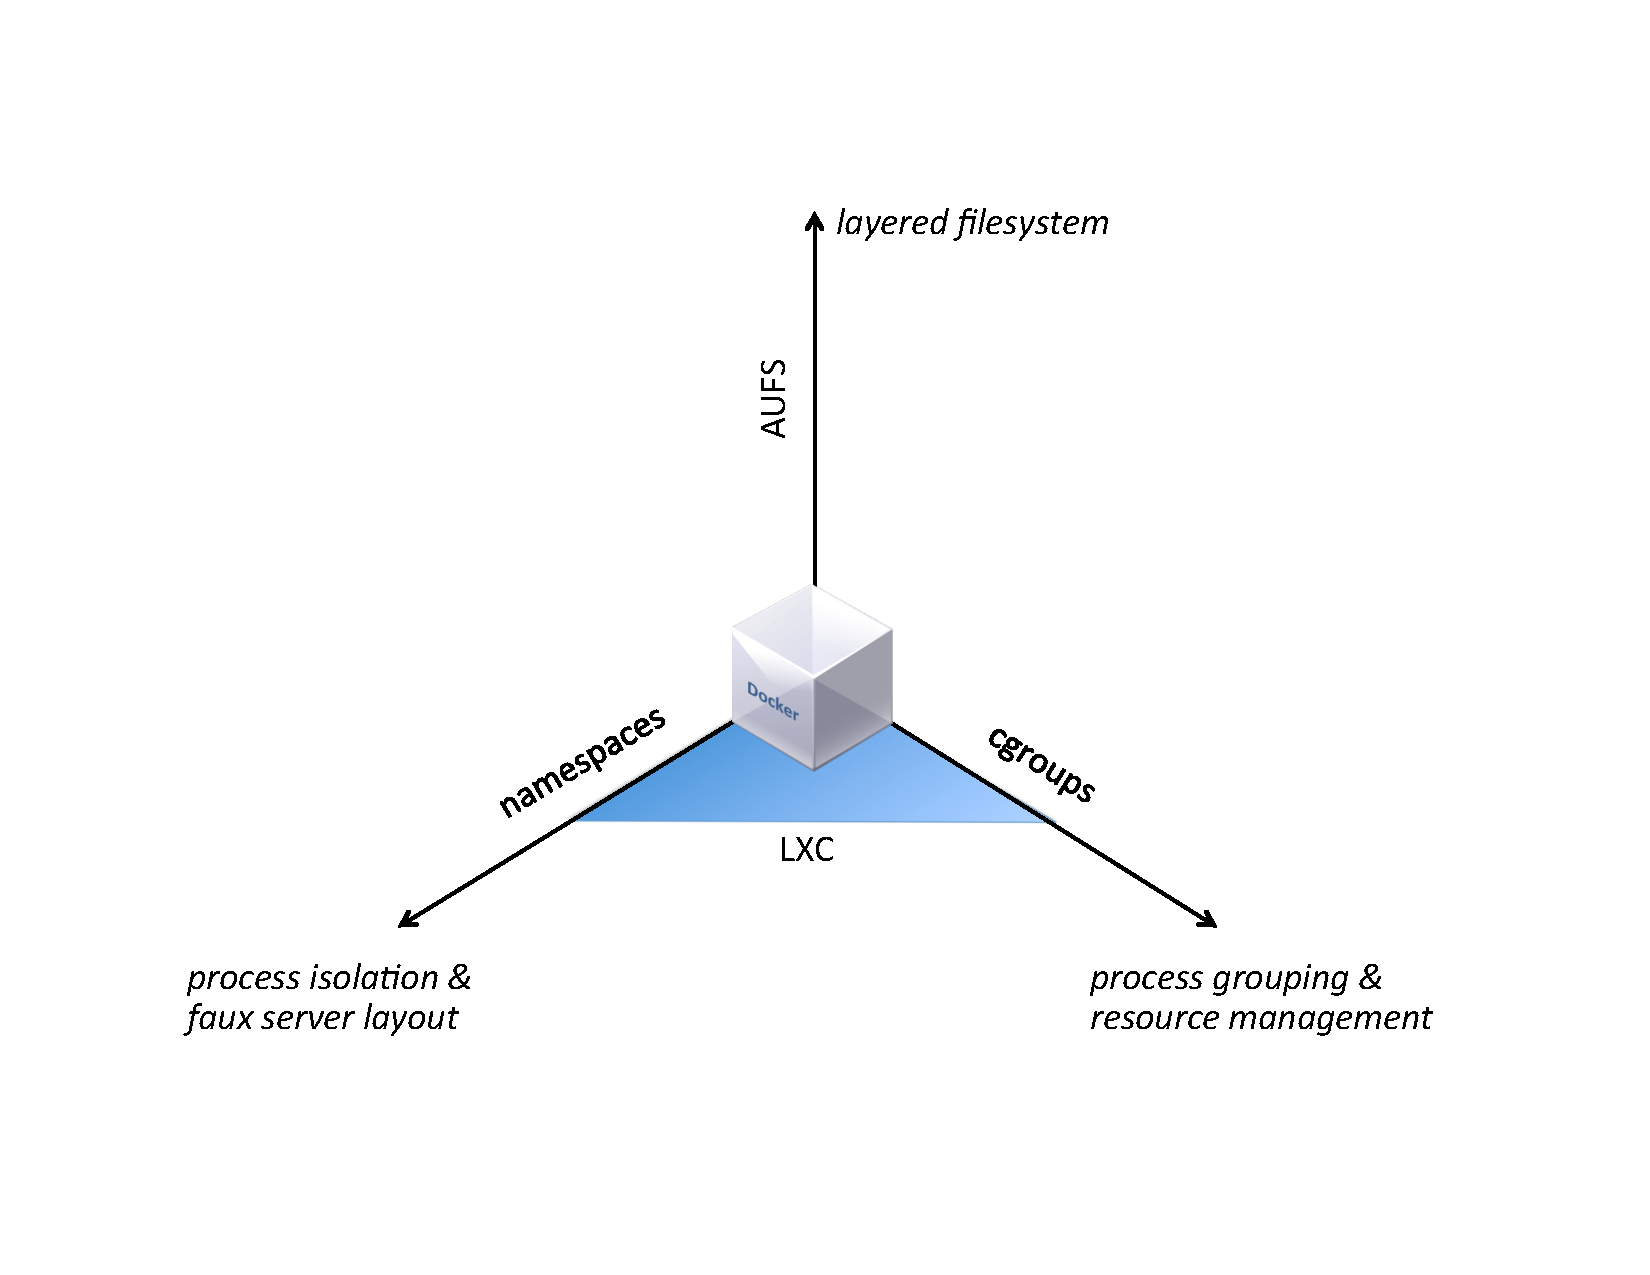
\includegraphics[width=1.0\textwidth]{docker.pdf}
    \caption{A graphic outlining the three fundamental components that make up the Docker framework. Namespace and cgroup support are provided by the LXC (LinuX Container) kernel extensions, and filesystem layering is provided by AUFS.}
\end{figure}

\subsection{cgroups}
Cgroups, or control groups, are a feature on the Linux kernel that provides resource limiting, in the form of memory or disk limits, as well as prioritization of CPU and disk throughput. These features are comparable to those offered by a virtual machine hypervisor to allocate a given amount of memory and CPU, network, and disk priority to a virtual machine.

\subsection{namespaces}

Namespaces are the mechanism by which each Docker container is isolated from the host and other containers. There are many different namespaces that LXC supports, but probably the two most significant ones are the \texttt{pid} and \texttt{net} namespaces. The \texttt{pid} namespace is responsible for giving each container its own isolated environment for processes. A given container can only see and send signals to the processes that are running within the same container. In addition, the \texttt{net} namespace allows different containers to have what appears to be distinct network interfaces, thereby permitting two containers to simultaneously bind to the same port, for example \cite{lxc}.

\subsection{Another Union FileSystem (AUFS)}
AUFS, Another Union FileSystem, is the primary means through which Docker achieves both storage savings and faster deployments of containers. Each image inherits from a sequence of other images, up to the base image, and represents the set or sequence of changes on the filesystem. This layering of filesystems and images accomplishes two main benefits. First, it allows for a high degree of storage savings. If two containers are running the same OS and share some libraries and dependencies, the majority of their filesystems will only be represented once on disk and are not duplicated. Second, when downloading and deploying a container, if a host already has previous layers of the filesystem on which a given container depends, it need only download the incremental changes.

\subsection{Docker Registry}
Docker provides a public registry to which developers can push their custom Docker images and share their creations with others \cite{dockerregistry}. It has support for creating private images, but requires the user to pay to have more than one privately hosted image.

Docker also has open sourced the Docker Registry \cite{dockerregistry-github} to allow for privately hosted registries. For enterprises, this is a superior solution that allows for easy deployment and configuration of Docker containers across a wide area datacenter.

\section{Technical Terms}\label{ch2:lingo}
The comprehension of a few terms related to Docker is essential to the understanding of this thesis. 
\subsection{Dockerfile}
A Dockerfile, similar to a Makefile, is composed of a set of instructions used by Docker to build an image. It typically starts with an inheritance line, specifying from which image to inherit. This can either be a base image, or another image that has been previously built. After the inheritance instruction, the rest of the Dockerfile consists of a combination of commands to run, files to add, environment variables to set, and ports to expose. The Dockerfile can then be passed into the Docker engine, along with an optional tag, and the resulting image is built. Each command in the Dockerfile represents a new layer on the file system. Each change is performed, copy-on-write, such that the entire image ancestry is accessible at any time.

\subsection{Base Image}
A base image is a special kind of Docker image that does not have a parent image. The base image instead represents the set of files that make a given operating system unique, excluding the kernel. Examples of base images are Ubuntu 14.04 and CentOS7. Base images do not have a parent and instead fully represent an entire OS on their own. Base images are used as starting points from which all other projects can inherit \cite{baseimage}. 

\subsection{Containers vs. Images}
Images are read-only layers on the filesystem. Each layer is a distinct image. To run a container, one specifies an image and a command to run. All changes to the filesystem go to the top-most container layer of the filesystem, preserving all image layers beneath. Figure~\ref{ch2:imagevcontainers} illustrates all of these concepts.

\begin{figure}[h]
\centering
    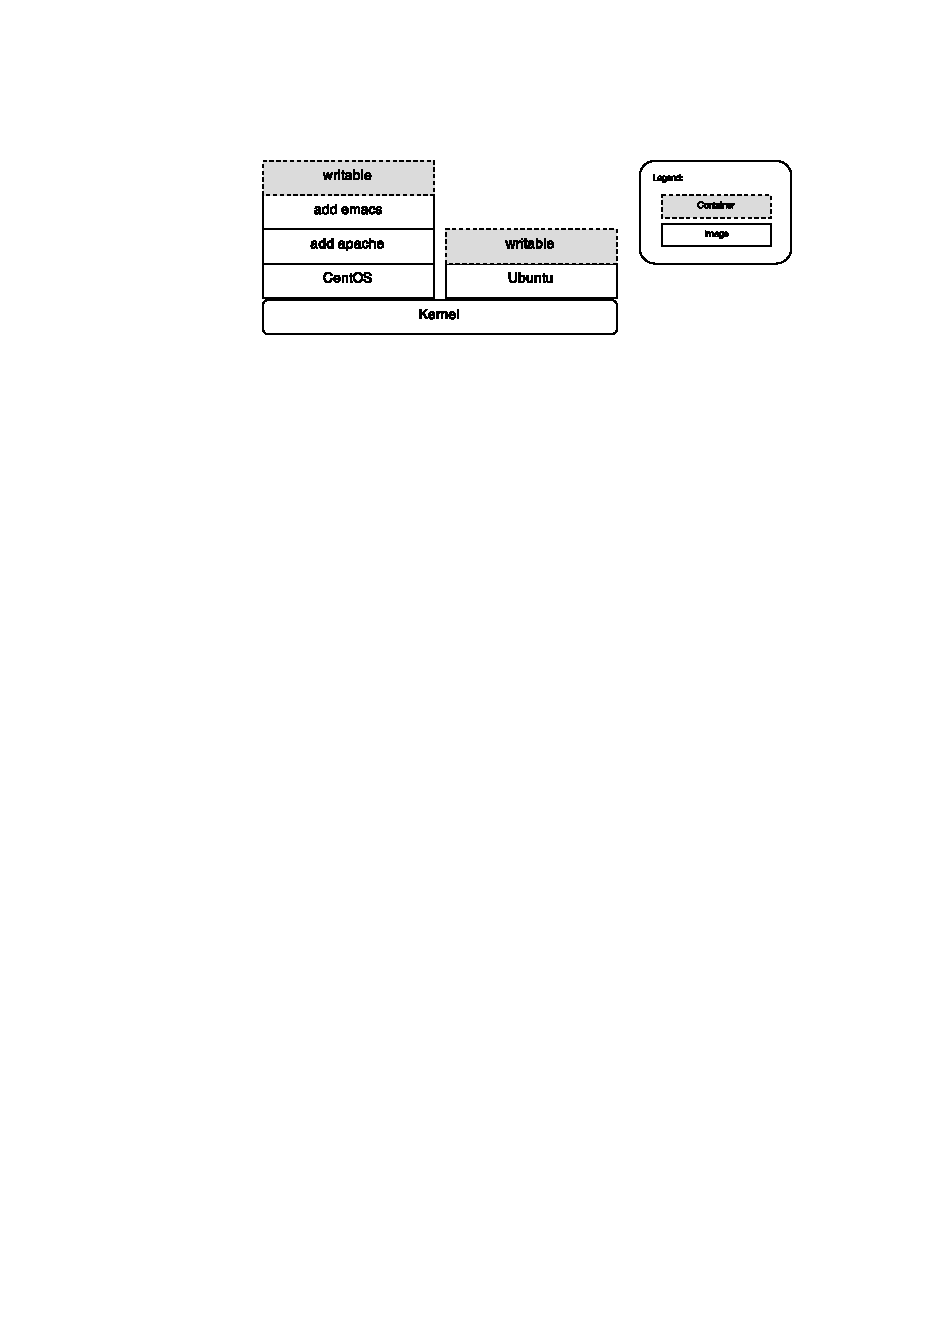
\includegraphics[width=1.0\textwidth]{cvimage.pdf}
    \caption{A graphic providing examples of the difference between containers and images in the Docker Engine. Containers are the top-most writable layers of the filesystem and represented by the rectangles with dashed lines and grey background. Images are the read-only layers used for inheritance and are represented by the rectangles with the solide lines and white background.}
\label{ch2:imagevcontainers}
\end{figure}

\section{Use Cases}\label{ch2:usecase}
\subsection{Cloud}
This is the primary target for which VM2Docker is geared. As an alternative to hosting virtual machines in the cloud, many cloud providers now offer the option to either directly use containers, run containers within a container-optimized VM, or both.

\subsection{DevOps}
Another essential audience for the Docker framework is the DevOps paradigm. DevOps is the process by which a piece of software is developed and subsequently deployed, along with the continuous revision process of simultaneous development and deployment. Historically, DevOps has been challenging to get right because of all of the dependencies a certain piece of software might have. During deployment, the software installed on a given developer's host must also be installed on the host running the deployed application. Docker provides a streamlined way to guarantee that a piece of software running on one host will run exactly the same on another host, as long as each host has the Docker Engine installed. This guarantee is an invaluable asset and is touted as the "first true" DevOps tool \cite{devops}. Ops managers may choose to deploy the Docker containers in the cloud or in their own private cluster of Docker-supported machines.

%\subsection{Benefits \& Drawbacks}\label{ch2:bd}
%https://news.ycombinator.com/item?id=8167928

\section{Industry Hype}\label{ch2:industry}

The hype over Docker, both in the open-source community as well as in the industry, has been unprecedented. In the past year and even more recently in the past six months, a number of influential players in the cloud hosting industry have begun to offer native support for running Docker containers. Specifically, Amazon has launched its own EC2 container service \cite{aws} and Google has their own container engine powered by the open-source cluster manager Kubernetes, Additionally, VMware, initially perceived to be threatened by container technology, has announced a partnership with Docker which attempts improve the overall user experience \cite{vmware}. In addition to the established cloud providers, other providers such as Tutum and Orchard, which was acquired by Docker, have been created that focus specifically on container deployment in the cloud. The excitement and popularity of the Docker framework across the industry is a testament to its utility and novelty as compared to the prior industry standard, virtual machines.

\subsection{Comparison to Virtual Machines}
While it remains to be seen whether Docker poses an immediate threat to the virtual machine landscape, it is evident that virtual machines and containers are distinct products that aren't necessarily direct competitors. Each caters to a slightly different audience.

Since Docker shares the kernel with the host, it only supports Linux-based containers and immediately discards support for legacy enterprise software that might need a Windows environment to run.

Central to the distinction between container and virtual machine is the tradeoff between density and isolation. Virtual machines offer the strongest form of isolation, comparable to that offered by physically separated hosts. Containers, on the other hand, share the kernel with the host, and therefore provide a much larger attack surface through which an attacker might be able to compromise another container on the same host. 

By giving up isolation, unlike virtual machines which incur a performance overhead, containers achieve near native performance as compared to running directly on the host itself \cite{performance}. Furthermore, the density of containers on a given host can be much higher than that of VMs. 

\begin{figure}[h]
\centering
\subfigure[Docker Container]{%
  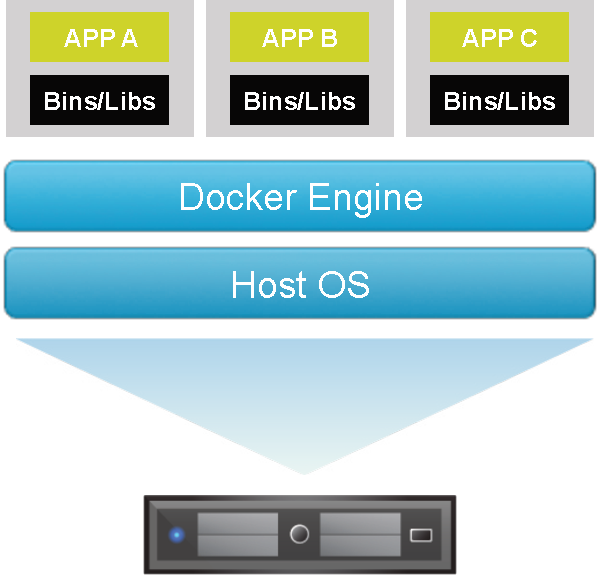
\includegraphics[width=.4\linewidth]{docker_h.pdf}
  \label{fig:sub1}}
\quad
\quad
\subfigure[Virtual Machine]{%
  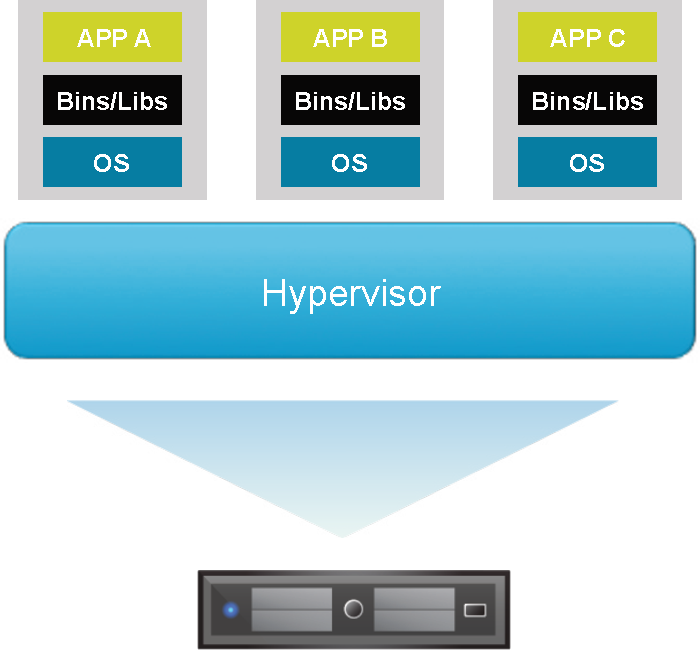
\includegraphics[width=.4\linewidth]{vm_h.pdf}
  \label{fig:sub2}}
\caption{A comparison of the components and isolation of virtual machines as compared to Docker containers. Each container consists of only an application and its dependencies and shares the underlying kernel with the host OS.}
\label{fig:test}
\end{figure}

Since Docker can run directly inside of a virtual machine, but not vice versa, there are interesting ways in which Docker and VMware VMs might be able to work together in the future to offer a streamlined experience that captures the benefits of each. Multiple, trusted, containers running in the same VM, for example, could provide stronger isolation while still achieving the portability and deployment benefits that Docker containers provide.

Another distinct advantage of VMs is there ability to perform live migrations from one host to another. VMware dubs this process vMotion\cite{vmotion}, and it is used as a direct building block for VMware's Dynamic Resource Scheduling (DRS)\cite{DRS}. Docker containers, unless running in a VM (and migrated with vMotion), cannot be live migrated to another host and instead must be shut down, moved, and started back up. CRIU\cite{CRIU} is a project under heavy active active development that attempts to bring this live migration to the container ecosystem by implementing checkpoint/restore functionality for Linux in userspace. Once completed, CRIU might be used as a primitive for dynamic resource scheduling among different Docker host. However, as of this writing, no such feature exists.
\subsection{Competitors}
Docker is one of the most successful and popular frameworks for container technology. However, there are also a number of other alternatives that are also built on top of Linux containers. 

\subsubsection{Flockport}
Flockport is a young alternative to Docker that focuses on entire virtualization workloads, instead of app delivery. As a result, Flockport does not boast the same kind of layered filesystem as Docker and instead is built on top of the LXC protocol \cite{flockport}.

\subsubsection{Spoonium}
Spoonium is a platform that attempts to bring container technologies to platforms not necessarily based on Linux. It touts many of the features of the Docker framework. Interestingly, Docker, too, has announced its intention of bringing Docker support to the Windows platform. Thus, it remains to be seen of Spoonium will experience the same kind of success that Docker has.

\subsubsection{Rocket - CoreOS}
Rocket, by CoreOS, is an alternative to Docker under heavy active development. CoreOS initially provided complete support for Docker, and their operating system was specifically built as a bare-bones operating system with the minimal amount of software installed to run Docker. A variety of disputes over the overall product vision has inspired CoreOS to develop their own take on containers, called Rocket, and we will see what sort of improvements and following this gets in the coming months and the software matures \cite{rocket}.

\subsubsection{Ubuntu - LXD}
One final player in the container field is Ubuntu and their announcement of LXD. LXD aims to build on top of LXC and serve as a hypervisor for containers. A main feature it aims to support is the live snapshotting of containers through CRIU\cite{CRIU}, which also enables them to support live migration of containers between hosts. These features are invaluable and would serve as an essential addition to the container framework, thereby bringing some of this container technology inline with that offered by VMware and vMotion and DRS \cite{vmotion,DRS}. Since LXD will work on a slightly lower level of the stack than Docker, it is possible it will also serve as an enhancement, rather than a direct competitor, to Docker \cite{lxd}.

%\subsection{Orchestration}





%% This is an example first chapter.  You should put chapter/appendix that you
%% write into a separate file, and add a line \include{yourfilename} to
%% main.tex, where `yourfilename.tex' is the name of the chapter/appendix file.
%% You can process specific files by typing their names in at the 
%% \files=
%% prompt when you run the file main.tex through LaTeX.
\chapter{Related Work}
\label{chap:relatedwork}
In this chapter, we discuss existing research in the fields relating to both container alternatives and conversion mechanisms. The existing work in this field is fairly limited, and to the extent of our research there is no existing tool that attempts to automate the conversion from VM to container. Everything must be done manually. Nevertheless, there are a few exist tools, as well as terminologies that are important in our overall discussion.

In sections~\ref{sec:dockerimport} and~\ref{sec:dockercommit}, we introduce two tools built into the Docker engine and describe why they are insufficient for the VM conversion process. Then, in section~\ref{sec:dockerize} we describe the term "dockerization" and how it is currently used in the industry. In section~\ref{sec:pvc} we mention Parallels Virtuozzo Containers and their connection to Docker. Finally, in section~\ref{sec:dtovm} we describe the alternative conversion, from Docker to Virtual Machine.

\section{Docker import}
\label{sec:dockerimport}
Included with Docker is the import tool that has the following documentation:\\

\texttt{Usage: docker import URL|- [REPOSITORY[:TAG]]}

\texttt{Create an empty filesystem image and import the contents of the tarball (.tar, .tar.gz, .tgz, .bzip, .tar.xz, .txz) into it, then optionally tag it.} \\

Theoretically, this tool would permit us to create a tarball out of a full-fledged virtual machine and import it directly into Docker. However, doing so would completely abandon the notion of layering different filesystems together to construct an image, and the final Docker image would take up the same space as the original virtual machine. Furthermore, if multiple virtual machines were converted in this manner, even if they had the same underlying OS and distribution, their layers wouldn't share any of the same lineage. Thus, two docker images would take up the same amount of space as the original two VMs. 

As a result, Docker recommends that this tool be used only to create base images. Base images should be made as small as possible and intuitively should only contain the necessary files to provide a fully-functioning OS. Packages can subsequently be installed on top of the base image depending on the desired function of the container. 

\section{Docker commit}
\label{sec:dockercommit}
Also, included with Docker is the import tool that has the following documentation:\\

\texttt{Usage: docker commit [OPTIONS] CONTAINER [REPOSITORY[:TAG]]}

\texttt{Create a new image from a container's changes} \\

As previously mentioned, a container represents the top-most writable layer of the filesystem, while images are the read-only layers from which a container can inherit. In the course of a container's lifetime, as changes are accrued, one can optionally choose to save these changes to a read-only layer, to be used in future images or containers, by using the \texttt{docker commit} tool.

\section{"Dockerization"}
\label{sec:dockerize}
Dockerization is the process of converting an application to be capable of being run within the Docker framework. Existing containers that run nginx, apache, or mysql, for example, are said to have been "Dockerized" from their original forms. This process generally consists of someone picking a framework or tool for which there is no publicly available Docker image. Then a Dockerfile can be generated that provides instructions on how to build the corresponding environment for the software. Finally, the Dockerfile and any associated files are shared to the public Docker registry, allowing other users to download and build these images for private use. The mapping from application to container is by no means automatic and generally one must manually write the instructions in the Dockerfile. 

Of particular importance is the distinction between making use of \texttt{docker commit}, as mentioned in section~\ref{sec:dockercommit}, as compared to creating a Docker image that is built purely from a set of instructions in a Dockerfile. Docker commit is not accepted as a valid Dockerization tool because it masks the exact changes made to the filesystem layer and generally results in Docker images that take up more space than if one were to build the same image from a set of instructions. 

In fact, Docker has recently started labeling "trusted builds" as those in the registry for which there is a complete set of instructions of how they are built in a publicly accessible GitHub repository. The builds are "trusted" in the sense that the complete set of instructions of how each image is built is observable by all potential users. 

Thus, VM2Docker aims to streamline the Dockerization process by offering the automatic and large-scale conversion of VMs to their corresponding Docker containers. We specifically focus on the filesystem layering process for evaluation and we do not make use of the ~\texttt{docker commit} tool in favor of greater transparency of the set of instructions used to build each image.

\section{Parallels Virtuozzo Containers (PVC)}
\label{sec:pvc}
Parallels is one of the few existing solutions that provides a seamless conversion from containers to virtual machines, and vice versa. Parallels' container solution is called Virtuozzo Containers and differs largely from Docker. However, the underlying idea of a more lightweight version of a virtual machine still remains. Parallels' \texttt{pmigrate} tool is a command-line utility that provides the seamless conversion between the two types of formats.

Interestingly, as of December 15, 2014, Parallels has abandoned their Virtuozzo Container format in favor of the Docker container format for their Cloud Server \cite{pvcloses}.

%\section{Docker Desktop}
%https://blog.docker.com/2013/07/docker-desktop-your-desktop-over-ssh-running-inside-of-a-docker-container/

\section{Docker $\to$ VM}
\label{sec:dtovm}
Unlike the task of converting VMs to Docker, the converse is extremely straightforward. Since Docker can be run within a VM, one can simply run the same Docker container within a VM to obtain a Docker image that has been ``converted" to a VM.
%% This is an example first chapter.  You should put chapter/appendix that you
%% write into a separate file, and add a line \include{yourfilename} to
%% main.tex, where `yourfilename.tex' is the name of the chapter/appendix file.
%% You can process specific files by typing their names in at the 
%% \files=
%% prompt when you run the file main.tex through LaTeX.
\chapter{VM2Docker}
\label{chap:vm2docker}
In this chapter, we outline the design and implementation of the VM2Docker system. In section~\ref{sec:usecases}, we discuss typical use cases for VM2Docker. In section~\ref{sec:sysoverview} we outline and diagram the system as a whole. The system itself consists of two major components: filesystem conversion, as discussed in section~\ref{sec:fsconversion}, and process detection, as described in section~\ref{sec:pdetection}. Finally, we conclude with a brief discussion of the system's technical specifications in section~\ref{sec:techspecs}.

\section{Use Cases}
\label{sec:usecases}
Overall VM2Docker has a number of theoretical and practical use cases where it might be particularly effective. We target single and multi-purpose virtual machines that run standard, unprivileged processes. Notably, the primary prerequisite is that any process or application running in the VM must also be able to function correctly in a headless Linux container. This excludes GUI applications, although they could theoretically be supported through a tool such as Docker Desktop \cite{ddesktop}. This also excludes any VMs that use custom modifications to the kernel or have privileged access to special devices on the host. As of Docker 1.2, custom privileges can also be added to containers to parallel those specified for a given VM on a case by case basis, but this generally breaks the complete isolation that Docker provides between containers.

Examples of such virtual machines that would be capable of being converted to a container are the following:
\begin{itemize}
\item Web server
\item Database
\item Mail server
\item Git server
\item Hadoop node
\item Cluster or grid computing node
\item Other non-UI computing
\end{itemize}

In all of these cases, VM2Docker will succeed in converting a given set of hosts to their corresponding, automatically layered Docker images. The goal of the layering is to maximize the size and quantity of layers that are shared in common among the different virtual machines. Since Docker retains just one copy of each layer on disk, regardless of how many images use the layer, the total disk space used by the converted containers will be less than that used by the original VMs. Furthermore, when run, the containers will achieve performance benefits of running on the lightweight Docker framework as compared to their original, fully-isolated and less performant VM environments. A full analysis and evaluation of the improved disk usage of VMs converted with VM2Docker is provided in chapter~\ref{chap:eval}.

%\section{Usage \& Configuration}
%%%%%%%%%%
\section{System Overview}
\label{sec:sysoverview}
In this section, we outline the design and implementation of the VM2Docker framework. The filesystem conversion process is broken down into three important steps. First, as outlined in section~\ref{sec:osdetection}, we determine the OS and distribution running on each VM and matches it up with a given Docker base image. Second, as described in section~\ref{sec:packagemanagement}, we assemble one or more additional layers corresponding to the packages that are installed in each VM. Finally, we apply a diff-based algorithm to create a layer that contains all other files that haven't yet been accounted for but were on the original VM filesystem. The next component of the VM conversion process consists of container configuration. VM2Docker automatically determines which processes are running on each host, along with the commands to run them, and maps them to commands to be run in a corresponding Dockerfile. Exposed ports are automatically detected and opened on the given containers, and container resources are allocated based on the resources present in the initial VM.

\begin{figure}[h]
\centering
    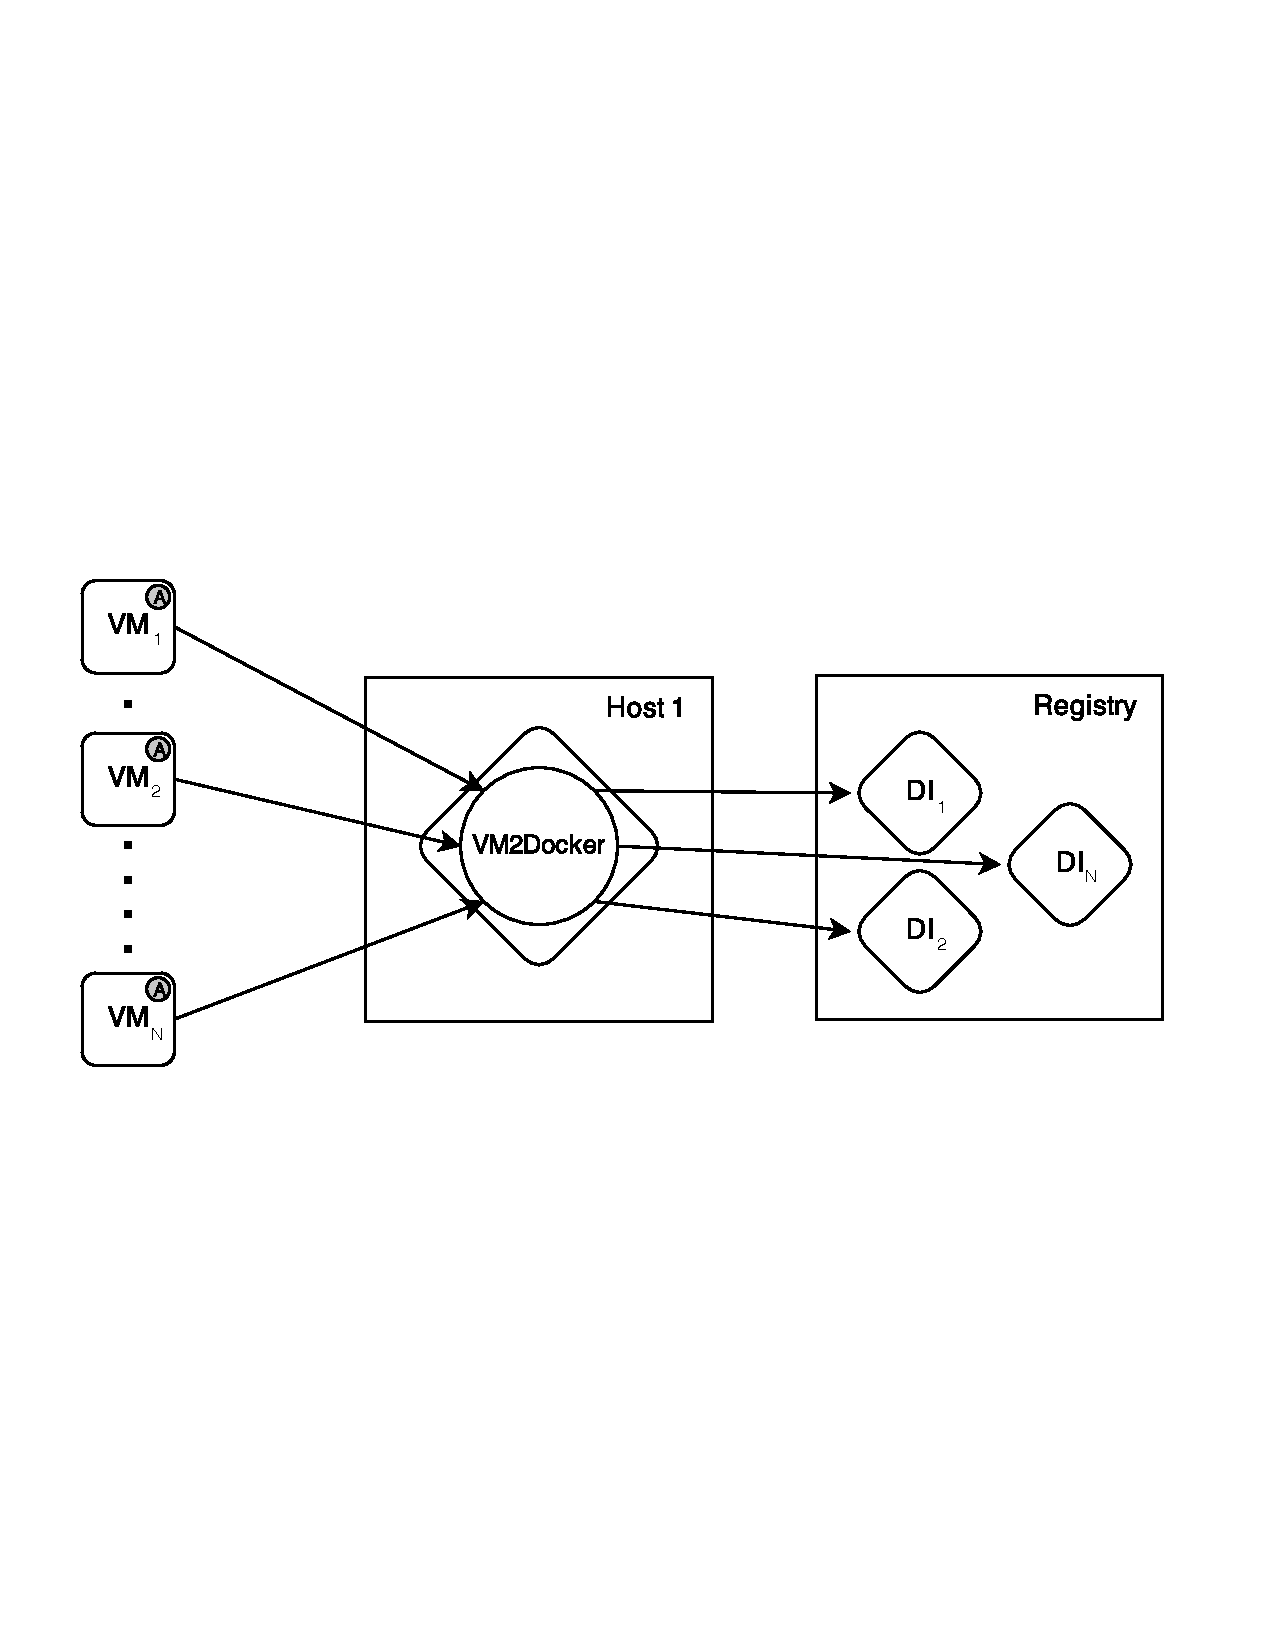
\includegraphics[width=1.0\textwidth]{system2.pdf}
    \caption{The following diagram illustrates an overview of the system and how the VM2Docker framework interacts with the virtual machines provided as input and converts them to corresponding Docker images. The rounded squares represent the input virtual machines and the rounded diamonds represent the resulting Docker images. To be converted, each VM must be running an instance of the "agent", as described in section~\ref{sec:agent}, and identified by a gray circle with the letter "A." The "chief," which initiates the conversion and is identified by the circle labeled VM2Docker, is itself a Docker image and can therefore be run on any host that has Docker installed. The resulting Docker images are deployed to a Docker registry, which can either be hosted on Host 1 or a separate host entirely. }
   \label{fig:sys}
\end{figure}
\subsection{Chief + Agent}
\label{sec:agent}
As displayed in figure~\ref{fig:sys}, the VM2Docker framework is divided into two components: the chief and the agent. The chief is centrally deployed on a single server which initiates the conversion. The agent is a self-contained executable that is deployed and run on each VM that needs to be converted. The chief communicates with the agent on each VM in order to convert them to their corresponding, layered, Docker images.  

\section{Filesystem Conversion}
\label{sec:fsconversion}
A significant component of this endeavor comprises the optimal decomposition of a virtual machine into a set of configuration files and an associated Dockerfile, which together can be used to build a Docker image. Docker`s filesystem layering allows multiple images that inherit from the same parent image to share many of the same files, therefore drastically cutting down on the total space needed for many copies or minor derivations of the same base image. In addition to space savings, the corresponding Docker images take up a fraction of the space of a VM and can therefore be downloaded and shared in a much more convenient manner.

Starting from the original VM, VM2Docker will apply a set of transformations in order to decompose the VM's filesystem into a set of layers, which, together, make up the original filesystem. At the end of the automatic layering process, a filesystem diff is created and applied from the topmost Docker layer to the original VM filesystem. This ensures that after the diff is applied, the Docker image is byte for byte equivalent to the original VM's filesystem. Figure~\ref{fig:layering} depicts how three such virtual machines, all running the same operating system and release, might share certain layers in common after being converted to the Docker format.

\begin{figure}[h]

\centering
    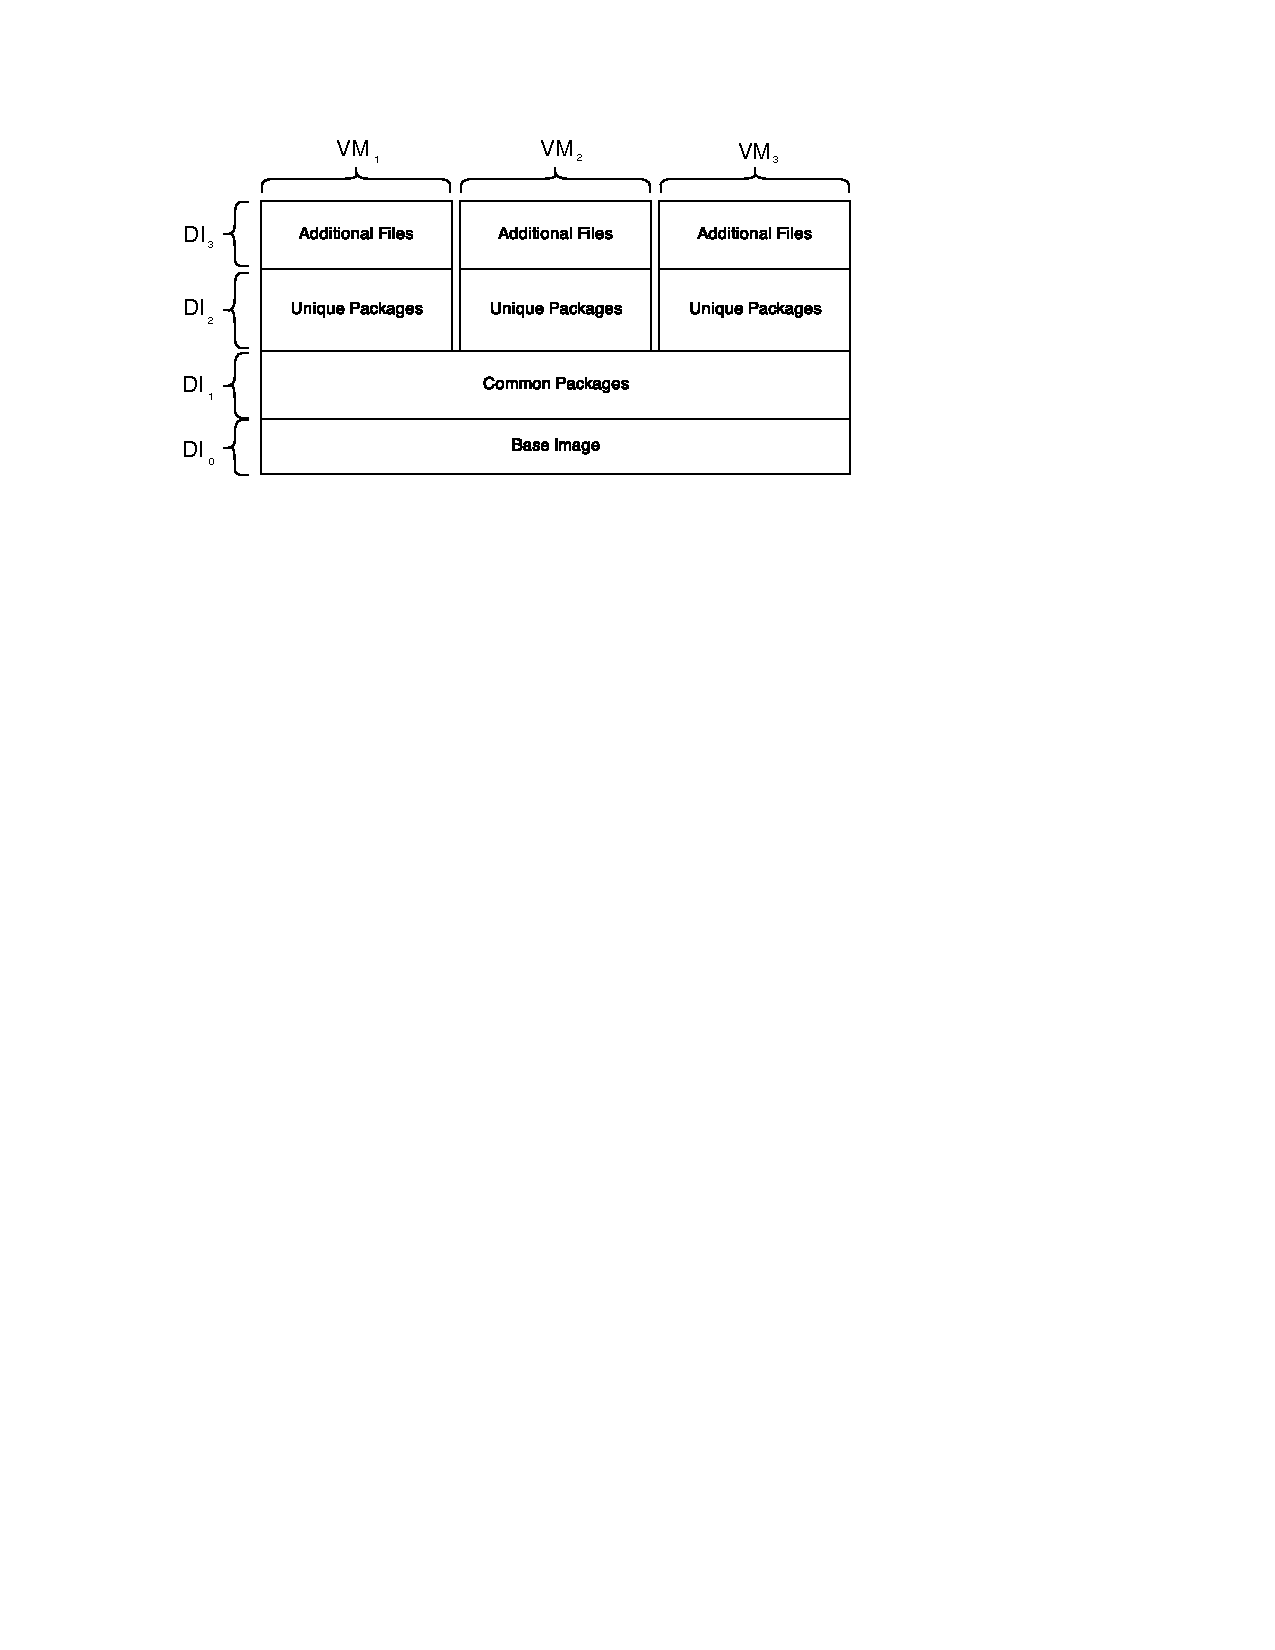
\includegraphics[width=0.7\textwidth]{layering.pdf}
    \caption{An example of how VMDocker layers the filesystems of three virtual machines running the same operating system and release. Docker will keep only one copy of layers $DI_0$ and $DI_1$, because each of the three VMs share these in common.}
\label{fig:layering}
\end{figure}

\subsection{Base Image}
\label{sec:osdetection}
The most straightforward way of exploiting layering in Docker is by means of simple Docker image inheritance. Built into the engine is a method by which each image can be told to start from an existing image, identified by a repository and tag name. This could either be a base image corresponding to a specific release of an operating system, or it could be a more complex image, which itself inherits from another image.

We make use of this layering by automatically detecting the distribution and release of the corresponding VM. As long as the VM is running a release of Linux with a kernel version that exceeds 3.8, it should be supported by VM2Docker. The distribution and release can be found in \texttt{/etc/*-release} and roughly correspond to the repository and tag name, respectively. Once obtained, we check for the existence of the corresponding base image on the Docker Registry. For now, we are using the publicly available registry but intend to transition to a private registry. A private registry would allow any such base images that are not available on the public registry, like RedHat because of licensing reasons, to be generated on the fly with a tool like \texttt{debootstrap} \cite{debootstrap} and then pushed to the registry for future availability.

\subsection{Package Management}
\label{sec:packagemanagement}

To increase the number of layers and maximize the sharing of these layers across different Docker images, we make aggressive use of package detection and installation. Each OS has a slightly different package management tool, so VM2Docker abstracts out the particular commands for a given tool and is therefore extensible regardless of the operating system in use. We have tested and implemented code that works for Ubuntu, Mageia, and CentOS, which use \texttt{apt-get}, \texttt{urpmi}, and \texttt{yum}, respectively.

We maximize layers in common by first computing the intersection of packages for all VMs of the same operating system and release. This set of packages is culled using dependency detection, which is described below. Once filtered, a Dockerfile is constructed that inherits from a given base image and contains instructions to install all packages in common.

This process is repeated a second time for each VM using the remaining packages that have not yet been installed. A Dockerfile is generated that inherits from the image created in the previous step and installs the remaining packages specific to this VM. Note that if there is only one VM of a given operating system and release, these two layers will be the same.

Presumably, the package installation process will consist only of package installs, but it is conceivably possible that there are some installed on the base image, but not the VM, which would lead to a Dockerfile instruction to uninstall the given packages.

The goal of this technique is to coerce the Docker image filesystem to be as similar to the original VM as possible before calculating the diff, thereby reducing its size.

\subsubsection{Dependency Detection}
\label{sec:depdetection}
A useful feature of VM2Docker that greatly reduces the number of packages installed and increases Dockerfile readability is its ability to reduce the number of packages listed to be installed within a given Dockerfile without affecting correctness.

Many packages installed on a given OS are never directly installed. Instead, they are installed as a result of satisfying a dependency for another package. In other words, even if explicit instructions to install these packages are not given, the end result is the same. VM2Docker takes advantage of this observation and the resulting improvements are incredibly effective, as shown in the evaluation section in table~\ref{table:culling}.

To accomplish this dependency-safe reduction in packages, we generate a directed graph of all the packages that will be installed, where there is an edge from $A$ to $B$ if and only if package $A$ depends on package $B$. Once generated, the only packages that need to be directly installed are those that have an in-degree of 0 or are a part of a strongly connected component of size greater than 1. The addition of the strongly connected component requirement takes into account the possibility of dependency cycles, in which packages will have an in-degree of greater than 0 but still must be included in the install list. See figure~\ref{fig:depgraph} for a visual representation of such a directed graph.

\begin{figure}[h]
\centering

    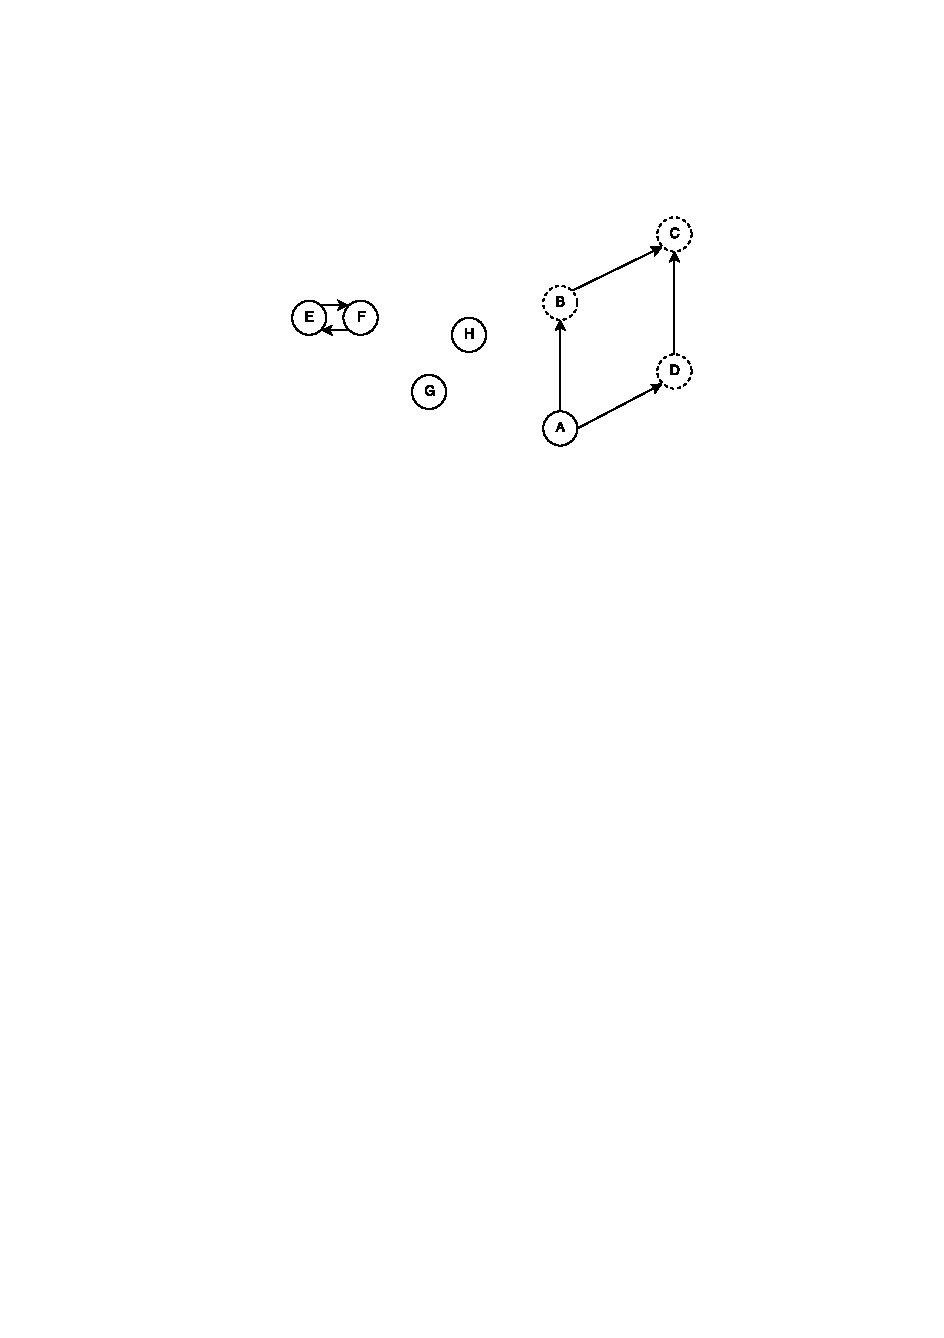
\includegraphics[width=.6\textwidth]{depgraph.pdf}
    \caption{In the example above, packages $A$-$G$ are pictured. Package $X$ depends on package $Y$ if and only if there is a directed edge from $X$ to $Y$. Of those pictured, packages $B$, $C$, and $D$ do not need to be installed because during installation of package $A$, the package manager will detect that $B$ and $D$ are uninstalled dependencies, and that $C$ is recursively a dependency of them. Packages $E$ and $F$ still need to be included, even though their in-degree is bigger than 0, because they are a strongly connected component on which no other installed nodes depend. All those packages that are removed from the list of packages to be installed are pictured with a dashed line circle, while the packages that can't be removed are pictured with a solid line circle.}
   \label{fig:depgraph}
\end{figure}

\subsection{Diff}
\label{sec:diff}
The topmost layer of the Docker image consists of all the files needed such that the entire filesystem is byte-by-byte equivalent to the original VM filesystem. This is accomplished by calculating a filesystem diff from the existing Docker image, with all packages installed, to the original VM filesystem. The Dockerfile is given instructions to inherit from the Docker image completed in the previous step, equipped with all packages installed, and then to apply the diff to the filesystem, thereby recovering the complete VM filesystem. There are a number of different strategies for computing this diff, each with its own benefits and drawbacks. We analyzed two in particular: \texttt{rsync} and \texttt{rdiffdir}, and VM2Docker is fully extensible to support other algorithms with very little user intervention and a simple subclass.


\underline{rsync}\\
\texttt{rsync} is a backup tool used to sync changes to and from a remote server. It can also be used between directories on the same host. Two rounds of rsync are needed in order to account for additions and modifications, as well as deletions. The first round, from Docker image to the VM filesystem, represents all of the changes and additions that need to be added to the Docker image to get to the VM. The second round, which we run in reverse, gives us the set of changes and deletions that have been applied. Cross-referencing these lists, we extract just the deletions and convert them to a list of the filepaths of the deleted files. We create a tarball of all of the changes and additions. To build the final Docker image, we expand the tarball and then iterate through the list and delete each file listed. This yields the filesystem of the original VM. 

\texttt{rsync} has the benefit of being a native C executable that is bundled with almost  every Linux system. The one major drawback is how it handles file modifications. Since the diff is represented as a set of files in directories, it has no way of indicating which components of a file have changed without copying the modified file in its entirety. This can be especially wasteful if a large file has only a few bytes modified. While the \texttt{rsync} algorithm is optimal about remote backups in only sending the changed version of a file and patching it on the other side, running \texttt{rsync} for two directories on the same host does not have the same sort of optimizations.

\underline{rdiffdir}\\
\label{sec:rdiffdir}
\texttt{rdiffdir} is a tool based on \texttt{rdiff} but that can be used for directories as well. The \texttt{rdiff} tool is an independent implementation of the \texttt{rsync} algorithm that generates delta files that can then be used to patch the existing file without the target file present. For example, if \texttt{rdiff} generates a delta file from $A$ to $B$. \texttt{rdiff} can use the delta to patch $A$ and recover file $B$, even if $B$ is no longer present. The \texttt{rdiff} algorithm uses a fixed size window to generate rolling hashes of a given file in order to generate these deltas in an optimal manner.

Use of \texttt{rdiffdir} generally allows for more optimal, smaller diffs to be created, thereby resulting in more portable Docker build instructions. The one major drawback of using \texttt{rdiffdir} is its non-native implementation. As a component of the Duplicity framework, \texttt{rdiffdir} is written in Python and therefore has some pre-existing dependencies. While the generating of the Delta file happens within the VM2Docker chief environment where dependencies are less important, the patching of the filesystem using the generated delta occurs in the resulting Docker container environment. If a given VM did not already have it installed, \texttt{rdiffdir} would need to be installed, the patch applied, and then uninstalled, which is a lot less straightforward than the expansion of a tarball as seen in the \texttt{rsync} example.


\subsection{Dockerfiles}
The instructions to build a given Docker image are provided in a corresponding Dockerfile. Starting from the base image, which we will call $DI_0$, VM2Docker generates a Dockerfile with a set of instructions that denote how to generate the next layer, given the current one. Figure~\ref{fig:dockerfiles} depicts this progression of Docker images, and how the Dockerfiles ($DF$) bridge the gap between them.

\begin{figure}[h]

\centering
    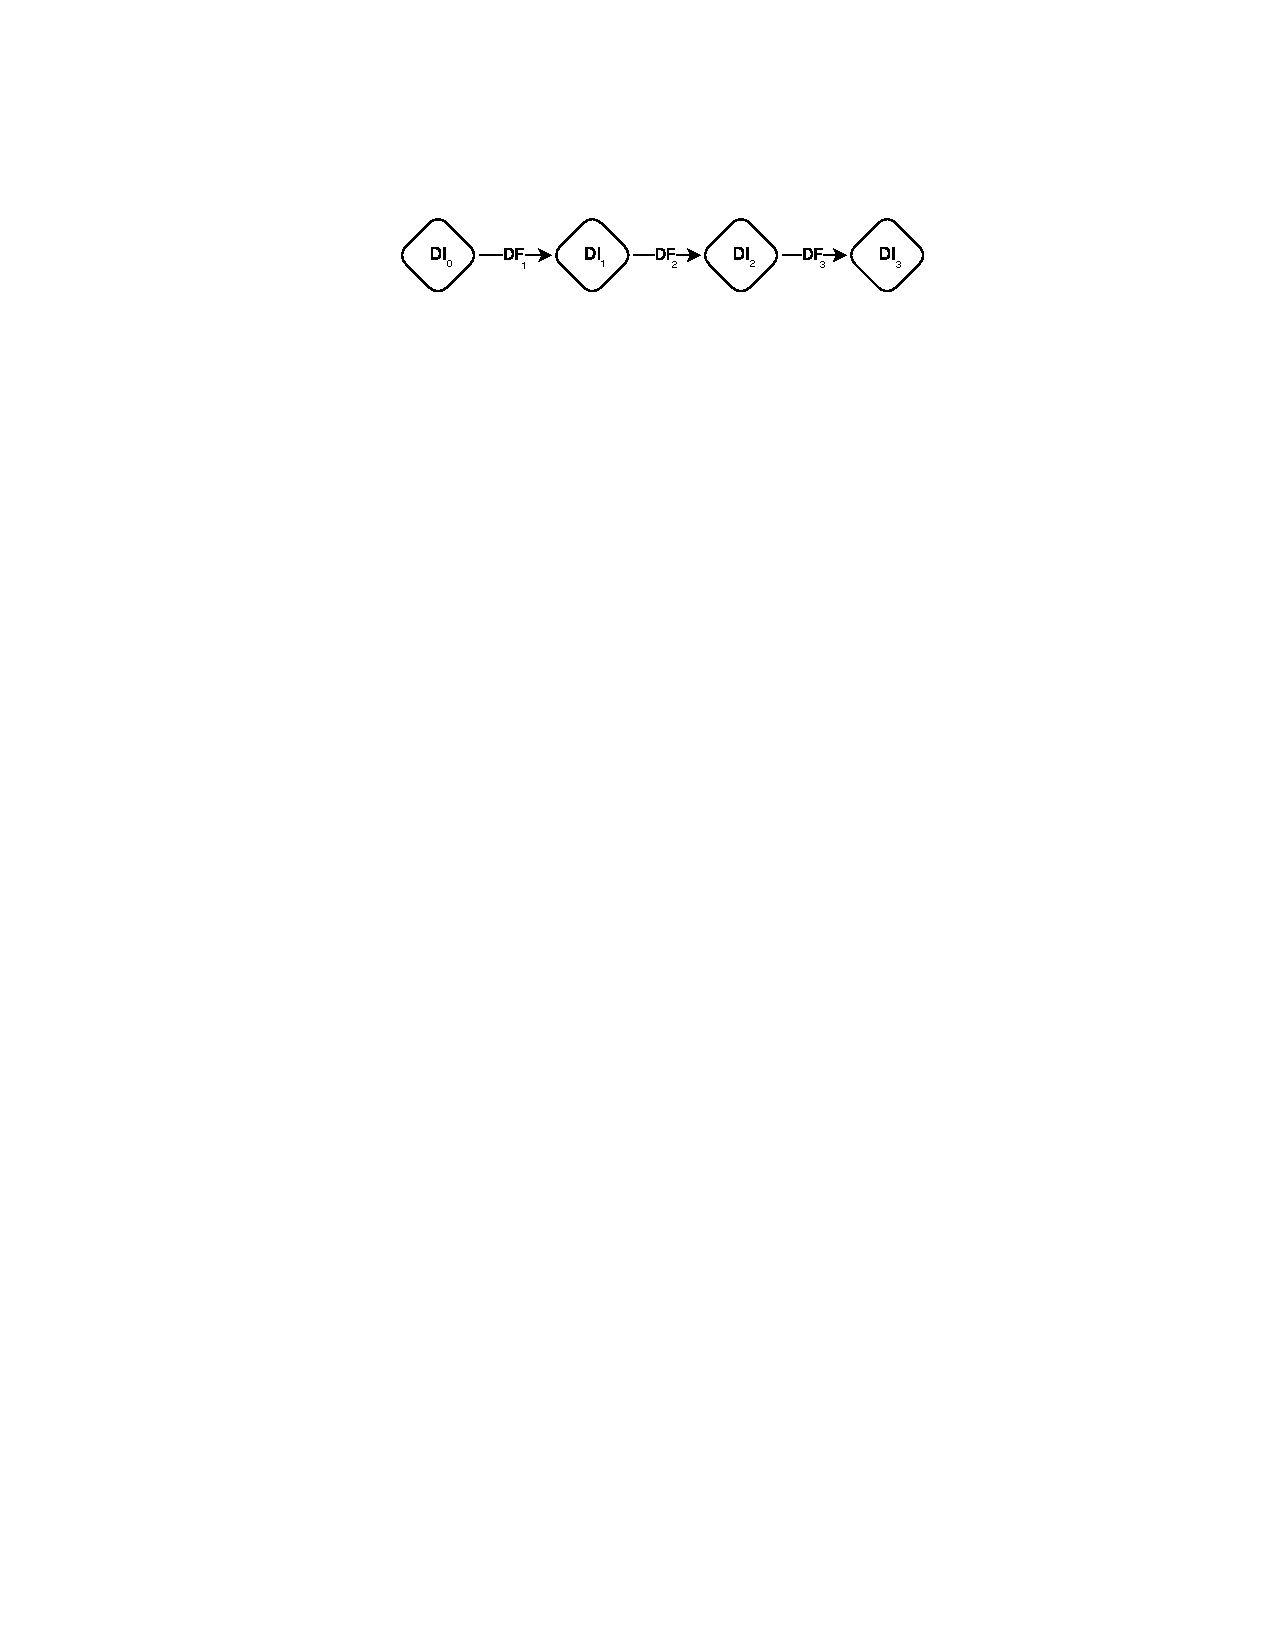
\includegraphics[width=0.7\textwidth]{dockerfiles.pdf}
    \caption{An example of the Docker image build process and the set of instructions used to get between images. Starting from the base image, $DI_0$, Docker generates image $DI_1$ by executing instructions contained in $DF_1$.}
\label{fig:dockerfiles}
\end{figure}

Depending on the operating system and the diff algorithm specified, VM2Docker generates the appropriate commands and inserts them into the Dockerfiles, along with the auxiliary delta file in the case of $DF_3$. When built, the Docker images are generated and take the inheritance scheme as pictured in figure~\ref{fig:dockerfiles}.


\subsection{Verification}

With all of these filesystem transformations in place, it is essential to verify that the Docker image that is built is identical to the original VM in terms of its filesystem. Since the diff operation is always executed last, the resulting patch should always restore the final filesystem to be a byte-for-byte identical copy as the original VM filesystem. Even if the process of installation or uninstalling packages selects the wrong ones, the worst that can happen is an increase in the size of the diff layer, which does not affect the correctness of the system.

For completeness, we implement an optional flag that can be enable a verification tool to be run with the virtual machine conversion. After conversion is complete, it will build the final Docker images and export them to disk. The resulting Docker images are identical to the VM if and only if the filesystem diff between the Docker image filesystem and the original VM filesystem is the empty set.

\subsection{Additional Space-Reducing Techniques}
\label{sec:addnltechs}
Certain files in the VM are either unnecessary, or can be regenerated on the fly. Since Docker containers share their kernel with the host operating system, they disregard any kernel modules that are provided in the container. Thus, we can safely remove these associated files from the diff in order to save space. Furthermore, the package repository cache takes up a fair amount of space, and is used only for performance reasons. This can be safely purged from the filesystem without affecting correctness. For Ubuntu, these files are located at \texttt{/var/cache/apt/pkgcache.bin} and \texttt{/var/cache/apt/srcpkgcache.bin} and can potentially take up about 100 MB.

\section{Process Detection}
\label{sec:pdetection}
In addition to converting the filesystem to one that may better exploit layering, another big component of VM2Docker is its ability to automatically configure the resulting containers in a manner similar to that of the original VM.

Unlike VMs which start up an entire operating system, Docker containers are started by running a specific command in the shell. VM2Docker maps each running process on a host to a new container. In this paradigm, the command that runs the container corresponds to the command to start up the given process, and each VM may potentially map to multiple containers. Although technically feasible, VM2Docker may not always work with multi-process VMs, depending on the level and type of interprocess communication occurring between the isolated processes. Further research into multi-container orchestration is discussed in section~\ref{sec:future}.

The VM2Docker agent, which runs directly on the host with root privileges, can automatically detect the currently running processes that were kickstarted at startup, as well as the commands used to start them using \texttt{ps}. Furthermore, we use \texttt{netstat} to determine which processes are bound to which ports, to be sure to expose the corresponding ports through Docker. The agent also reads information available in the \texttt{proc} pseudo-filesystem in order to determine the current working directory and environment variables of the given process. All of this information is transmitted to the chief over a socket and is used during the container configuration component of the conversion process.

Finally, in terms of resource allocation, the VM2Docker agent reads from the \texttt{/proc} pseudo file-system and parses the information available in \texttt{meminfo} and \texttt{cpuinfo}. This information is passed over a socket to the VM2Docker chief during conversion in order to provide the container with the same resource restrictions and allocations as its corresponding VM.

\section{Technical Implementation \& Specifications}
\label{sec:techspecs}
The VM2Docker chief is written as a Python script and is made to communicate with one or more VM2Docker agents. Each agent is a simple executable, written in C, and is compiled to the appropriate architecture and OS, depending on the VM. The C agent sets up a TCP socket through which the chief can communicate via a custom remote procedure call protocol. This protocol is responsible for transmitting the entire filesystem, checking app dependencies, and getting specific runtime information about the process that will be running within the container. In order to be platform independent, the VM2Docker chief is bundled with an associated Dockerfile such that the conversion process happens within Docker container. This allows for all dependencies to be automatically and seamlessly installed. The entire conversion process is therefore platform agnostic and requires only the Docker environment as well as a target Docker host and/or registry to store the newly created Docker images and optionally run them. Thus, VM2Docker makes use of Docker's ability to run inside of itself \cite{dockerindocker}. Prior to making this design decision, an early prototype of VM2Docker instead took as argument the filepath to the root of the VM's filesystem. This required a separate VM to be running the same operating system as the VM to be converted, which proved unwieldy for each additional operating system attempted. Furthermore, since we had only access to the filesystem, process detection was not possible either. The current chief and agent design overcomes both of these challenges. 

An additional technical challenge was determining the protocol to be used to respond to remote procedure calls to the agent over the socket. These calls returned both plain text, as well as raw data in the case of the filesystem transmission, of arbitrary length back to the chief for processing. To handle the incoming data, we designed a reusable ring buffer in Python with a seamless interface that provided methods for reading until a specified single or multi-byte delimiter. The protocol we chose makes use of the null byte as a delimiter for text. In the case of a file, a header is sent that specifies the number of bytes to read after the header, while ignoring any occurrences of the delimiter. This abstraction allowed us to effectively and seamlessly handle the transmission of data from agent to chief.

\subsection{Usage}

%TODO: technical challenges


The prototype of VM2Docker is available at \url{https://github.com/ecbtln/vm2docker}.
%% This is an example first chapter.  You should put chapter/appendix that you
%% write into a separate file, and add a line \include{yourfilename} to
%% main.tex, where `yourfilename.tex' is the name of the chapter/appendix file.
%% You can process specific files by typing their names in at the 
%% \files=
%% prompt when you run the file main.tex through LaTeX.
\chapter{Evaluation}
\label{chap:eval}
All evaluation was done on a Mid 2012 15 inch MacBook Pro with 2.7 Ghz Intel Core i7 processor and 16GB of RAM, equipped with a solid state drive (SSD). All VMs were running on the same host, though VM2Docker makes no such restriction in practice, as only the IP address of each VM is required. The practical convenience of running on the same host allowed for a drastic speed improvement when transferring the entire VM's filesystem over the socket from agent to chief, as opposed to over a potentially slower network connection.

In section ......., ....., ....

\section{Evaluation Strategy}
When attempting to evaluate the performance and effectiveness of the VM2Docker framework, we must first describe the variables of interest and the overall benefits of the Docker container format. The most explicit benefits, as introduced in chapter~\ref{chap:docker}, are those related to the performance benefits, as well as portability, of the Docker format. Since Docker containers are more lightweight than their VM counterparts, containers are much quicker to startup and have generally less performance overhead and are more comparable to running directly "native" on the host. As a result of this improved performance, hosts can also support a higher density of running containers as compared to the corresponding virtual machines.These benefits are universal to the Docker framework and are not in any way affected by the specifics of the VM2Docker framework. Therefore, we acknowledge that these benefits are essential and must be considered when deciding whether to use virtual machines or Docker containers, but that they will not be directly quantified when evaluating the effectiveness and performance of the VM2Docker system as a whole.

One of the other major benefits of the Docker framework is a consequence of its unique, layered filesystem. When containers are built, stored, and deployed, the Docker Engine makes aggressive use of caching of previous layers in order to improve build and deployment time. For example, if a Dockerfile used to generate a Docker image has already been built and is then modified by the addition of one more command at the end of the file, the Docker Engine will not need to rebuild the entire Docker image from scratch. Instead, it will automatically recognize that all layers up to the last one have already been built (and cached), and it can quickly generate a new image just by layering one command on top of the already existing Docker image. In addition to build time, deployment time and storage space can also be greatly improved by the automatic layering provided by VM2Docker. As mentioned in section~\ref{sec:dockerimport}, without VM2Docker, the only automatic method of converting a VM to the Docker format is one huge layer, in its entirety, using the Docker import tool. Every time this container is deployed, the contents of the entire filesystem must be transmitted over the network from the Docker registry to the host wishing to run the container. This gets especially wasteful when multiple containers, imported from VMs, need to be deployed. Even if they are identical except for perhaps a few packages or other files that have been changed, the entire VM must be transmitted over the network to be deployed, and the additional Docker image takes up an identical additional amount of space as the original VM. 

As the number of layers and the sharing of these layers increase across multiple VMs, Docker has the ability to improve deployment time, by transmitting only the necessary layers, and overall space usage. This is the primary quantitative metric by which we evaluate the VM2Docker system across multiple releases of three different operating systems: Ubuntu, CentOS, and Mageia. We first focus on the conversion of a single VM and analyze the relative size of each layer in the resulting Docker image, with and without package detection. We look at the results of using the two aforementioned diff strategies (\texttt{rsync} and \texttt{rdiffdir}). Then, we expand the set of inputs to multiple virtual machines at a time, with varying amounts of filesystem contents in common across many different layers in order to analyze the space savings as a function of $N$, the number of virtual machines.

Additionally, we briefly discuss the benefits of minimizing the complexity of each Dockerfile as a function of the number of packages included for a given install instruction. As mentioned in section~\ref{sec:depdetection}, we present the results of the application of dependency detection on minimizing the length of a given package install list without affecting the resulting built Docker image.

We also spend some time qualitatively describing the process of making use of VM2Docker for these three distinct operating systems and their respective package management tools.

Finally, although we focus on the filesystem layer sizes that VM2Docker produces, we also briefly mention the time required to successfully convert and deploy a set of VMs to their Docker counterparts. These absolute numbers are less essential because the conversion must only proceed once. However, we still spend some time describing certain factors that may affect the conversion time, such as network throughput, hard drive speed, and the number of packages installed.



\section{Quantitative Results}
In the following section, we evaluate the quantitative results of the VM2Docker framework. Primarily, we focus on disk usage and the relative sizes of various different layers that VM2Docker creates. Next, we touch on the ability for VM2Docker to make use of dependency detection to cull the list of packages required to recover the original VM, in its entirety.

\subsection{Disk Usage}
The primary innovation of VM2Docker is the means by which it generates reusable, stackable layers that are automatically employed by Docker to minimize space usage on a given host. Overall, the goal of layering is to allow a host to save space by keeping one copy of an entire sequence of images, no matter how many unique Docker images inherit from the same parent. Within this context, VM2Docker targets virtual machines that are running the same operating system and release and potentially share a lot of packages in common. VM2Docker automatically layers the virtual machines provided so that the Docker engine is able to optimally store only one copy of the common layers, regardless of how many unique Docker images (converted from virtual machines) may inherit.

Figure~\ref{fig:systemeval} shows an example of the four basic layers we try to create for every virtual machine ($DI_0$ through $DI_3$), where two of the four are shared among all virtual machines of the same operating system and release. The major pieces of state that are provided as input are the virtual machines (VMs) and their corresponding operating systems (OSs). The outputs of the VM2Docker framework are the diamonds, $DI_0$, $DI_1$, $DI_2$, and $DI_3$, which correspond to the base image, the common packages layer, the unique packages layer, and the additional files layer, respectively.

\subsubsection{Descriptions of State}

\underline{VM}\\
The VMs are the inputs provided to the library. They are fully functioning virtual machines with as many or as few packages and additional files installed as needed. They must be running a Linux-based operating system with kernel version $\ge$ 3.8. Any OS beyond that is theoretically supported; however, VM2Docker has been only tested to work with Ubuntu, CentOS, and Mageia. Support for additional OSs is achieved by subclassing the appropriate base class and overriding a small set of OS-specific commands and parameters.

\underline{OS}\\
Each OS is an operating system and specific release that corresponds to the set of VMs provided as input. Therefore $M \le N$. If all VMs provided as input are of the same operating system and release, then $M=1$. Ubuntu, CentOS, and Mageia were specifically chosen because the publicly accessible "Docker Hub" has base images available for many of the major releases of these operating systems.

\underline{Base Images}\\
Base images are watered-down versions of a given release of an Operating System and range in size between 100 and 200 MB. They do not contain the kernel. They are represented by $DI_0$ in the diagram

\underline{Common Packages}\\
The next layer, $DI_1$, consists of a given base image with the set of packages installed that are common to all VMs of a given operating system release in the set of VMs provided as input.

\underline{Unique Packages}\\
The next layer, $DI_2$, consists of the installation of additional packages, on top of the common packages, that are not in the intersection of software for a given operating system release.

\underline{Additional Files}\\
The final step in the conversion of files is performing a filesystem diff from the previous layer, $DI_2$ to the original 


\newpage
\newpage

\begin{figure}[h]

\centering
    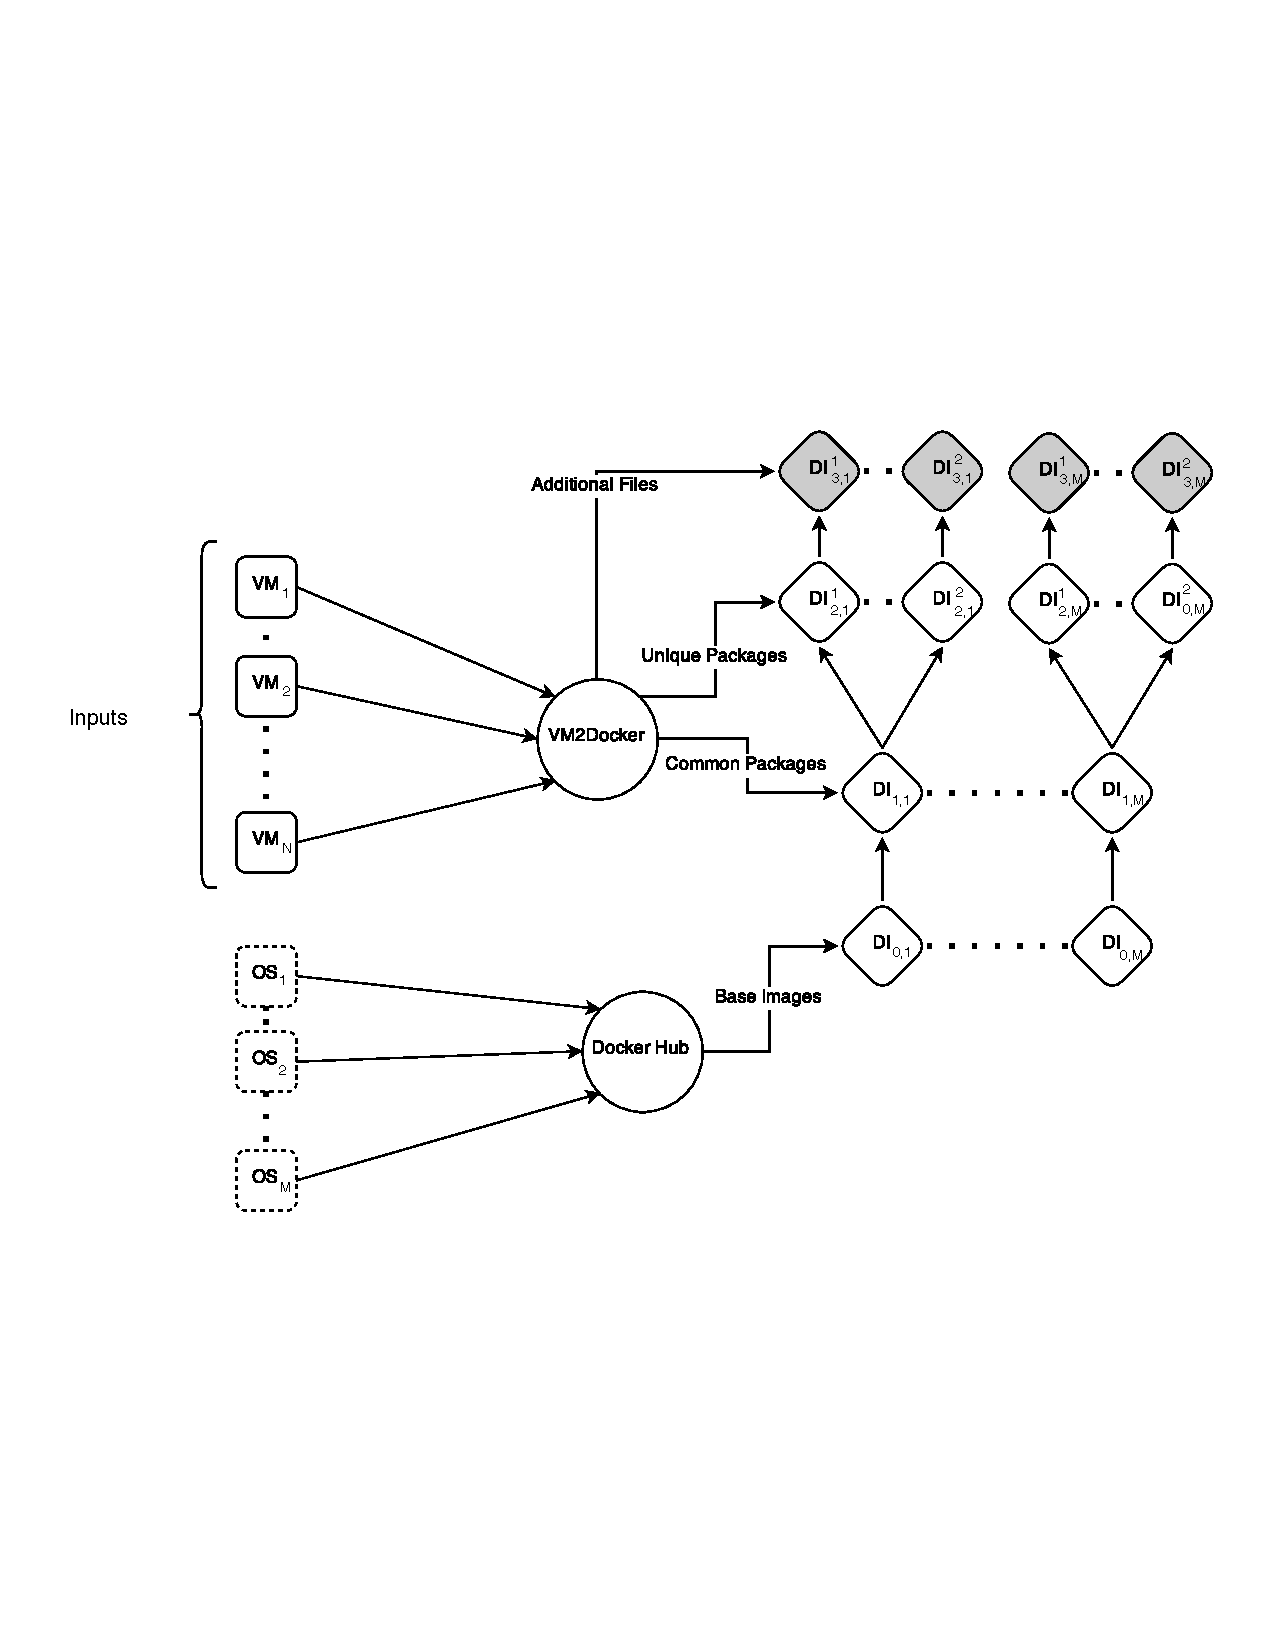
\includegraphics[width=1.0\textwidth]{system.pdf}
    \caption{The following diagram illustrates an overview of the system and how the VM2Docker framework interacts with the virtual machines provided as input and converts them to corresponding, layered, Docker containers. The rounded squares represent the input virtual machines, the circles correspond to immutable programs that interact with the inputs or outputs in some way, and the rounded diamonds represent the resulting Docker images. Each image consists of a series of layers, which is illustrated by starting at the given image and traversing the links backwards to the base image ($DI_0$). The final images, equal to the original VM filesystem, are represented by the shaded diamonds ($DI_3$). The number of these is exactly equal to N, the original number of VMs to be converted.}
\label{fig:systemeval}
\end{figure}
%$\text{DC}_3$)
% ($\text{DC}_0$)

\subsubsection{Single VM Conversions}
For the following set of experiments, we will assume that $N=1$ in the following diagram. By extension, this also implies that $M=1$. In practice, this reduces the effectiveness and utility of the system as a whole. As we will see, there is a tradeoff between increased layering and increased aggregate image size. VM2Docker generally favors the former at the expense of the latter, but the benefits of the former are not fully realized without multiple virtual machines present. As a result, converting a single virtual machine, while supported, is less optimal and is done purely as a theoretical analysis of the relative size of layers that VM2Docker can produce for a wide range of inputs.

We start by analyzing the results of running a single, vanilla install of a Linux operating system through VM2Docker with package management disabled. These virtual machine installers were obtained through the respective software websites are available for public download. With package management disabled, the view of layers produced for a given virtual machine is collapsed to $DI_0$ and $DI_3$. There is also a Dockerfile, which we will denote $DF$, that provides the instructions and additional data to the Docker engine of how to build $DI_3$ from $DI_0$. While the total size of $DI_3$ is by definition the same regardless of which diff algorithm is used, as we will see, the size of the delta file and therefore $DF$ can vary. Thus, the size of $DF$ and $DI_3$ are therefore important metrics in determining the speed of deployment and disk space required while running, respectively. We assume for the sake of consistency, that all sizes are provided, uncompressed. In practicality, the Docker engine likely automatically makes use of compression on both sides of a given download of an image. We therefore leave that topic as one beyond the scope of this paper and simply acknowledge this omission.

We use the term, bare VM, to denote a virtual machine, not including kernel files and other cache files that may be removed, as mentioned in section~\ref{sec:addnltechs}. This exclusion allows us to focus on benefits and drawbacks of our layering strategy without confounding the results of the strict benefits of excluding the kernel files, which would not be used inside of the Docker framework.

Tables~\ref{table:diff},~\ref{table:diff2}, and~\ref{table:diff3} show the results of these conversions. As we see, \texttt{rdiffdir} generally provides a slightly more compact delta file as compared to the \texttt{rsync} alternative. However, due to the dependencies of the \texttt{rdiffdir} package itself, as discussed in section~\ref{sec:rdiffdir}, the rsync algorithm is generally simpler and more straightforward to analyze. Furthermore, the byte representation of the the \texttt{rsync} diff file (a tarball of changes and modifications) maps directly to the size of $DI_3$, so it is simpler to use these interchangeably in our discussion.

In many cases, the aggregate size of all layers is no smaller than the original VM size. This implies that some increase in the size of $DI_0+DI_1 + DI_2$, $x$, results in a decrease in the size of $DI_3$, $y$, where $|x| \ge |y|$. These results are an example of the size to layering tradeoff mentioned at the beginning of this subsection. To better quantify this tradeoff, we introduce two important quantities that will be used throughout the evaluation process. 

First, we introduce a measure of the total space used in all layers up to and including layer $i$. This metric, $\Phi_i$, is defined as:

\begin{equation}
\Phi_i = \sum_{j=0}^i DI_j
\end{equation}

Throughout our discussion of single VM conversions without package management, $\Phi_1$ is the only additional value of interest, since $DI_2=DI_3=0$ so $\Phi_1=\Phi_2=\Phi_3$. When we incorporate package management, $DI_2 \neq 0$ and then with multiple VM conversions $DI_3 \neq 0$. These values will help quantify the fixed cost of increased layering at different locations in the inheritance tree for the first such VM to be converted. 

We also define a metric, $\Xi$, as the minimum whole number of VMs needed in order to achieve the goal of aggregate space savings. As we will see, $\Xi$ increases as we add more aggressive package management detection, but this also decreases $DI_3$, which can be thought of as the marginal cost of an additional VM of the particular OS and release. Theoretically, $\Xi$ can be defined at multiple layers of the inheritance tree, depending on which packages certain VMs share in common. For example, two VMs may share the same OS and release, and some but not all of the same packages installed. In this case, they would share $DI_0$ and $DI_1$ in common. In other cases, certain VMs might only differ in their filesystem composition, and could therefore share up to $DI_2$ in common. Thus, we consider $\Xi_i$ as the minimum whole number of VMs needed to achieve the goal of aggregate space savings, where the VMs share up to layer $i$ in common. This value can be attained by solving the following inequality for the smallest possible whole number value, $\Xi_i$.

In the equations below, we define $\beta$ as the size of the Bare VM.

\begin{equation}
\Phi_i + (\Phi_3 - \Phi_i)* \Xi_i \le \Xi_i * \beta
\end{equation}

However, for simplicity, we consider only this value when all packages are shared in common, and the $DI_3$ layer is different. Therefore, formally, $\Xi = \Xi_2$ can be simplified to the following:

\begin{align*}
\Phi_i + (\Phi_3 - \Phi_i)* \Xi_i &\le \Xi_i * \beta \\
\Phi_2 + (\Phi_3 - \Phi_2)* \Xi_2 &\le \Xi_2 * \beta \\
\Phi_2 + (DI_3)* \Xi &\le \Xi * \beta\\
\Xi &\ge \frac{\Phi_2}{\beta - DI_3} \\
\Xi &= \ceil*{\frac{\Phi_2}{\beta - DI_3}}
\end{align*}

%TODO!!: consider reorganizing equations to go before the start of the single VM conversions section

In the results, the layering tradeoff is very minimal while making use of only filesystem diffs. With $\Xi =2$ for all OS releases tested, we see that the presence of even a single additional container image of the same OS and release ensures that the layering strategy introduced by Docker not only breaks up the VM into more logical, deployable components but also saves space in the process.

\begin{table}[h]
\centering
    \begin{tabular}{| c | c | c | c | c | c | c |}
    \hline
& \multicolumn{5}{|c|}{\bfseries Ubuntu Server} \\ \hline
    \bfseries Release & \itshape 12.04 & \itshape 13.04 & \itshape 13.10 & \itshape 14.04 & \itshape 14.10 \\ \hline
    \bfseries Bare VM ($\beta$) & 1023.5 & 774.1 & 1055.2 & 1109.9 & 1029.9\\ \hline
    \bfseries Base Image ($DI_0$) & 99.1 & 160.4 & 174.6 & 192.0 & 196.9  \\ \hline
    \bfseries rsync & 956.7 & 730.9 & 963.6 & 1008.9 & 876.4\\ \hline 
    \bfseries rdiff & 934.4 & 738.2 & 957.3 & 971.2 & 872.5\\ \hline 
    \bfseries $\Xi$ & 2 & 2 & 2 & 2 & 2  \\ \hline
    \end{tabular}
\caption{The results of running VM2Docker with a single VM input and various releases of Ubuntu. The \texttt{rdiff} algorithm generall provides slightly smaller delta files. For all inputs, $\Xi = 2$ and therefore space savings begin to occur on the second instance of a given OS release.}
\label{table:diff}
\end{table}

\begin{table}[h]
\centering
    \begin{tabular}{| c | c | c | c |}
    \hline
& \multicolumn{3}{|c|}{\bfseries CentOS Minimal} \\ \hline
    \bfseries Release & \itshape 5* & \itshape 6 & \itshape 7 \\ \hline
    \bfseries Bare VM & 2441.5 &  573.7 & 779.4\\ \hline
    \bfseries Base Image ($DI_0$) & 496.0 & 236.1 & 243.1\\ \hline
    \bfseries rsync & 2190.0 & 478.1 & 601.8\\ \hline 
    \bfseries rdiff & 2138.7 & 416.7 & 519.4\\ \hline
\bfseries $\Xi$ & 2 & 2 & 2 \\ \hline
    \end{tabular}
\caption{The results of running VM2Docker with a single VM input and various releases of CentOS. The \texttt{rdiff} algorithm generall provides slightly smaller delta files. For all inputs, $\Xi = 2$ and therefore space savings begin to occur on the second instance of a given OS release.}
\label{table:diff2}
\end{table}

\begin{table}[h]
\centering
    \begin{tabular}{| c | c | c |}
    \hline
& \multicolumn{2}{|c|}{\bfseries Mageia} \\ \hline
    \bfseries Release & \itshape 3 & \itshape 4*  \\ \hline
    \bfseries Bare VM & 636.1 & 2706.1 \\ \hline
    \bfseries Base Image ($DI_0$) & 160.4 & 174.1\\ \hline
    \bfseries rsync & 525.1 & 2575.4\\ \hline 
    \bfseries rdiff & 511.0 & 2613.0\\ \hline 
\bfseries $\Xi$ & 2 & 2  \\ \hline
    \end{tabular}
\caption{The results of running VM2Docker with a single VM input and various releases of Mageia. The \texttt{rdiff} algorithm generall provides slightly smaller delta files. For all inputs, $\Xi = 2$ and therefore space savings begin to occur on the second instance of a given OS release. The * denotes that VM2Docker was run on the fullly featured release of this OS with all default packages installed, which explains the increase in overall size of the input VM.}
\label{table:diff3}
\end{table}

We next continue the analysis of these basic, vanilla linux VMs by enabling the use of package management. We therefore now also consider the size of an additional layer, $DI_1$, in our discussion. For simplicity, we assume we are only using \texttt{rsync} as our preferred method of filesystem diff, and label this $DI_3$.

As shown in tables~\ref{table:diffpm} and~\ref{table:diffpm2}, when package management is enabled in VM2Docker we observe a few important trends. First, the size of $DI_3$ decreases as a result of the existence of $DI_1$. This makes sense and is expected because the package management logic allows for some of the filesystem space occupied by packages that was formerly stored in the filesystem diff to be extracted downwards into $DI_1$. A consequence of this is that the total size of all layers, $\Phi_3$, also increases. However, overall this tradeoff is considered acceptable and preferred because $\Xi$ remains fixed at 2 and the overall layering and therefore deployability of each container increases.

When analyzing the overall results of these base case experiments and the layering results of converting a single virtual machine at a time, we take a step back and consider the efficiency of these results. An optimal conversion would be one such that the size of $DI_3$ is as close to 0 as possible. This would imply that the package extraction and reinstallation process is 100\% effective and is able to fully account for all or almost all files within a VM. The implications of such a container would be that the vanilla VMs would be fully "Dockerized." In practice, however, the size of $DI_3$ is far from zero, although the resulting sizes are still greatly reduced from the size of the original VM. There are a few practical limitations of the package detection and reinstallation process that can account for these results. Due to the automatic detection of packages and reinstallation on top of $DI_0$ with auto-generated commands, it is likely that some, but not all, of the packages that are reinstalled are not identical byte-for-byte versions of the original packages that were installed on the VM. This can be due to a difference in version number, release, or some other subtle difference in the installation process. This would result in some or all of a given package to still exist in the ``additional files" component of $DI_3$. There is also a host of software and files that can't necessarily be reinstalled from the default package management tool for the given OS. Cache files, too, can sometimes account for 50-100 MB of files in the original VM.

This point of comparison is used to quantify the marginal cost of deploying an additional VM, before and after the VM2Docker framework has performed the automatic layering. In tables~\ref{table:diffpm} and~\ref{table:diffpm2}, this value is represented by the symbol $\chi$ and is shown to range from 15.8 to 56.5.
 
% data tables that include package installation
\begin{table}[h]
\centering
    \begin{tabular}{| c | c | c | c | c |}
    \hline
& \multicolumn{4}{|c|}{\bfseries Ubuntu Server} \\ \hline
    \bfseries Release & \itshape 12.04 & \itshape 13.10 & \itshape 14.04 & \itshape 14.10 \\ \hline
    \bfseries Bare VM & 1023.5  & 1055.2 & 1109.9 & 1029.9\\ \hline
    \bfseries $DI_0$ & 99.1 & 174.6 & 192.0 & 196.9  \\ \hline
    \bfseries $DI_1$ & 227.3 & 273.7 & 194.9 & 271.7  \\ \hline
    \bfseries $DI_3$ & 862.2 & 733.7 & 894.8 & 687.6\\ \hline 
\bfseries $\chi$ & 15.8 & 30.5 & 19.4 & 33.2\\ \hline 
     \bfseries $\Phi_3$ & 1188.6 & 1182.0 & 1281.7 & 1156.2\\ \hline
\bfseries $\Xi$ & 2 & 2 & 2 & 2\\ \hline
    \end{tabular}
\caption{The results of running VM2Docker with a single VM input and various releases of Ubuntu. As the overall layering increases, the size of $DI_3$ decreases, which results in a increasing \% overall reduction, $\chi$ in the marginal cost of deploying a given VM. For all inputs, $\Xi = 2$ and therefore space savings begin to occur on the second instance of a given OS release.}
\label{table:diffpm}
\end{table}

\begin{table}[h]
\centering
    \begin{tabular}{| c | c | c | c |}
    \hline
& \multicolumn{2}{|c|}{\bfseries CentOS} & \multicolumn{1}{|c|}{\bfseries Mageia} \\ \hline
    \bfseries Release & \itshape 6 & \itshape 7 & \itshape 3 \\ \hline
    \bfseries Bare VM & 573.7 & 779.4 & 636.1\\ \hline
    \bfseries $DI_0$ & 236.1 & 243.1 & 160.4  \\ \hline
    \bfseries $DI_1$ & 286.5 & 417.1 & 544.2 \\ \hline
    \bfseries $DI_3$ & 381.9 & 339.9 & 465.9 \\ \hline
\bfseries $\chi$ & 33.4 & 56.5 & 26.8 \\ \hline
     \bfseries $\Phi_3$ & 904.5 & 1000.1 & 1170.5 \\ \hline
     \bfseries $\Xi$ & 2 & 2 & 2 \\ \hline
    \end{tabular}
\caption{The results of running VM2Docker with a single VM input and various releases of CentOS and Mageia. As the overall layering increases, the size of $DI_3$ decreases, which results in a increasing \% overall reduction, $\chi$ in the marginal cost of deploying a given VM. For all inputs, $\Xi = 2$ and therefore space savings begin to occur on the second instance of a given OS release.}
\label{table:diffpm2}
\end{table}


%TODO: discussion here about these threshold numbers for number of VMs for package management to make sense. etc. 


\subsubsection{Multiple VM Conversions}
\label{sec:multivm}
For the following set of experiments, we will assume that $M=1$ in figure~\ref{fig:systemeval}. This will greatly reduce the number of experiments to be run as well as simplify the understanding of the system diagram in each case. Each distinct operating system does not share any resulting image layers in common because the first layer, the base image ($DI_0$), is OS and release-specific. Thus, restricted our set of inputs such that all VMs share the same OS and release ($M=1$) does not drastically alter the results and instead represents a narrowing of scope to a single tree of image layers, pictured on the right in the diagram. The results for $M>1$ can be therefore obtained by merging the results from a set of $M$ independent experiments each of which $M=1$.

We therefore seek to analyze various combinations of VM inputs of a given OS and release, each with different package and file compositions. These results will provide material evidence for the theoretical calculations done in the previous section. In all experiments so far, it was determined that only a second additional VM was needed in order to establish total space savings as compared to not using the VM2Docker system at all. Thus, these multiple VM experiments, for simplicity, will only have 2 or 3 total VMs provided as input, but we argue that the scenarios chosen are highly representative of the types of combinations and subsets of VMs VM2Docker might need to handle. Furthermore, as the number of VMs of a given OS and release increases, the overall space savings will increase, as argued in the previous section.

It is very hard to describe what might be an "average" looking input to this system because one could use a virtual machine to do a wide range of computing. Nonetheless, there are many real-world practical use cases where VM2Docker might be particularly effective. The class of VMs that are used as servers in a simple client-server interaction are one example of such inputs. A given VM might be running a webserver, database, mail server, or other server-based daemon and might represent one such input to the VM2Docker system. 

We have designed a total of five experiments with various characteristics and combinations of input VMs in order to highlight strengths and weaknesses of the overall algorithm and framework. For each scenario, we begin by describing how we expect VM2Docker to handle these inputs in terms of the expected size of the outputs. These experiment descriptions will be OS-agnostic. We next present the results of running this experiment for specific releases of multiple OS's (Ubuntu, CentOS, and Mageia). Finally, we discuss any findings that might be unexpected or out of the ordinary.

\begin{enumerate}
\item \underline{Scenario A}\\
\textit{Input}:\\
$\boldsymbol{VM_1}$: Minimal OS, $\sim$ 1GB \textemdash\ $\boldsymbol{VM_2}$: OS Complete Install, $\sim$ 3GB\\

The difference between these two VMs is additional packages and repositories that are provided in the complete install. The second VM will contains all of the packages on the first VM, as well as a few gigabytes of additional software.


\textit{Expected Output}:
%$DC_1$: 286.5 MB\\
%$DC_2^1$: 0 MB\\
%$DC_2^2$: $\sim$ 1.5 - 2 GB\\
%$DC_3^1$: 157.1MB\\
%$DC_3^2$: 300-500MB\\

With two VMs provided as input, they will each share the same base image $DI_0$ for the given OS release. The next layer, $DI_1$, will also be common to the two containers and will contain all the packages common to the two VMs. At this point, the inheritance tree will split into two, one branch for each of the two provided inputs. $DI_1$ will be exactly the same size as the original $DI_1$ from the single VM experiments. $DI_2^1$ will be an empty layer that occupies no space, because there are no packages in $VM_1$ that are not also in $VM_2$. $DI_2^2$ will take up a few GB as it will be where all of the packages unique to $VM_2$ are located. Finally, $DI_3^1$ will be the same size as its corresponding layer in the original experiments and $DI_3^1$ we can expect to be larger as it will contain the remainder of the packages and their associated files not also installed in the previous layer.

\begin{table}[h]
\centering
    \begin{tabular}{| c | c | c | c|}
    \hline
    \bfseries Release & \itshape Ubuntu 13.10 & \itshape CentOS 6 & \itshape Mageia 3\\ \hline
    \bfseries $\boldsymbol{DI_1}$ & 273.7 & 226 & 248\\ \hline
    \bfseries $\boldsymbol{DI_2^1}$ & 0 & 129 & 147\\ \hline 
\bfseries $\boldsymbol{DI_2^2}$ & ?? & 129 & 147\\ \hline 
\bfseries $\boldsymbol{DI_3^1}$  & 733.7 & 129 & 147\\ \hline 
\bfseries $\boldsymbol{DI_3^2}$ & ?? & 129 & 147\\ \hline 
    \end{tabular}
\caption{The results of running the multi VM scenario A with M=1. All values are in MB.}
\label{table:multiscenarioa}
\end{table}



\item \underline{Scenario B}\\
\textit{Input}:\\
$VM_1$: CentOS6 Minimal, 676 MB\\
$VM_2$: CentOS6 Minimal plus 300 MB of additional files scattered across the OS, 1000 MB\\

\textit{Expected Output}:

%$DC_1$: 286.5 MB\\
%$DC_2^1$: 0 MB\\
%$DC_2^2$: 0 MB\\
%$DC_3^1$: 157.1MB\\
%$DC_3^2$: 457MB\\

The only differences between these two VMs comes in the addition of 300MB of files that can't be categorized into packages. This will result in an increase in $DI_3$ of the size of the additional files that were added to the VM.

\begin{table}[h]
\centering

    \begin{tabular}{| c | c | c | c|}
    \hline
    \bfseries Release & \itshape Ubuntu 13.10 & \itshape CentOS 6 & \itshape Mageia 3\\ \hline
    \bfseries $\boldsymbol{DI_1}$ & 205 & 226 & 248\\ \hline
    \bfseries $\boldsymbol{DI_2^1}$ & 67 & 129 & 147\\ \hline 
\bfseries $\boldsymbol{DI_2^2}$ & 67 & 129 & 147\\ \hline 
\bfseries $\boldsymbol{DI_3^1}$  & 67 & 129 & 147\\ \hline 
\bfseries $\boldsymbol{DI_3^2}$ & 67 & 129 & 147\\ \hline 
    \end{tabular}
\caption{The results of running the multi VM scenario B with M=1. All values are in MB.}
\label{table:multiscenariob}
\end{table}


\item \underline{Scenario C}\\
\textit{Input}:\\

$VM_1$: CentOS6 Minimal, 676 MB\\
$VM_2$: CentOS6 Minimal plus 300 MB of additional files scattered across the OS, 1000 MB\\
$VM_3$: CentOS6 Complete, 2.8 GB\\

\textit{Expected Output}:

%$DC_1$: 286.5 MB\\
%$DC_2^1$: 0 MB\\
%$DC_2^2$: 0 MB\\
%$DC_2^3$: $\sim$ 1.5 - 2 GB\\
%$DC_3^1$: 157.1MB\\
%$DC_3^2$: 457MB\\
%$DC_3^3$: 300-500MB\\

These results should be a combination of the two previous 2VM experiments, with the sizes remaining the same as if the experiments were run separately.
\begin{table}[h]
\centering

    \begin{tabular}{| c | c | c | c|}
    \hline
    \bfseries Release & \itshape Ubuntu 13.10 & \itshape CentOS 6 & \itshape Mageia 3\\ \hline
    \bfseries $\boldsymbol{DI_1}$ & 205 & 226 & 248\\ \hline
    \bfseries $\boldsymbol{DI_2^1}$ & 67 & 129 & 147\\ \hline 
\bfseries $\boldsymbol{DI_2^2}$ & 67 & 129 & 147\\ \hline 
\bfseries $\boldsymbol{DI_2^3}$ & 67 & 129 & 147\\ \hline 
\bfseries $\boldsymbol{DI_3^1}$  & 67 & 129 & 147\\ \hline 
\bfseries $\boldsymbol{DI_3^2}$ & 67 & 129 & 147\\ \hline 
\bfseries $\boldsymbol{DI_3^3}$ & 67 & 129 & 147\\ \hline 
    \end{tabular}
\caption{The results of running the multi VM scenario C with M=1. All values are in MB.}
\label{table:multiscenarioc}
\end{table}


\item \underline{Scenario D}\\
\textit{Input}:\\

$VM_1$: CentOS6 Minimal, 676 MB\\
$VM_2$: CentOS6 Complete plus 300 MB of additional files scattered across the OS, 3.1GB\\
$VM_3$: CentOS6 Complete, 2.8 GB\\

\textit{Expected Output}:

%$DC_1$: 286.5 MB\\
%$DC_2^1$: 0 MB\\
%$DC_2^2$: $\sim$ 1.5 - 2 GB\\
%$DC_2^3$: $\sim$ 1.5 - 2 GB\\
%$DC_3^1$: 157.1MB\\
%$DC_3^2$: 600-800MB\\
%$DC_3^3$: 300-500MB\\

These results should be similar in practice to the previous experiment as well. An interesting feature of VM2Docker will be exposed here as well. Since $DI_2^2$ and $DI_2^3$ are the same, they will be only represented once on disk by the same image. This is thanks to an implicit feature of Docker. Since VM2Docker generates Dockerfiles, which are instructions to generate the image, the Dockerfiles for $DI_2^2$ and $DI_2^3$ will be the same (the commands are the same and they are installing the same packages). VM2Docker sorts the list of packages being installed to ensure that the command in the Dockerfile is the same on subsequent runs. 

\begin{table}[h]
\centering

    \begin{tabular}{| c | c | c | c|}
    \hline
    \bfseries Release & \itshape Ubuntu 13.10 & \itshape CentOS 6 & \itshape Mageia 3\\ \hline
    \bfseries $\boldsymbol{DI_1}$ & 205 & 226 & 248\\ \hline
    \bfseries $\boldsymbol{DI_2^1}$ & 67 & 129 & 147\\ \hline 
\bfseries $\boldsymbol{DI_2^2}$ & 67 & 129 & 147\\ \hline 
\bfseries $\boldsymbol{DI_2^3}$ & 67 & 129 & 147\\ \hline 
\bfseries $\boldsymbol{DI_3^1}$  & 67 & 129 & 147\\ \hline 
\bfseries $\boldsymbol{DI_3^2}$ & 67 & 129 & 147\\ \hline 
\bfseries $\boldsymbol{DI_3^3}$ & 67 & 129 & 147\\ \hline 
    \end{tabular}
\caption{The results of running the multi VM scenario D with M=1. All values are in MB.}
\label{table:multiscenariod}
\end{table}

\item \underline{Scenario E}\\
\textit{Input}:\\

$VM_1$: CentOS6 Minimal, 676 MB\\
$VM_2$: CentOS6 Complete, 2.8 GB\\
$VM_3$: CentOS6 Complete plus 1 more package of negligible size, 2.8 GB\\

\textit{Expected Output}:

%$DI_1$: 286.5 MB\\
%$DI_2^1$: 0 MB\\
%$DI_2^2$: $\sim$ 1.5 - 2 GB\\
%$DI_2^3$: $\sim$ 1.5 - 2 GB\\
%$DI_3^1$: 157.1MB\\
%$DI_3^2$: 600-800MB\\
%$DI_3^3$: 300-500MB\\

These results will be the same as in the previous experiment, except that $DI_2^2$ and $DI_2^3$ will no longer occupy the same space on disk and will be two distinct images. This reveals a shortcoming of VM2Docker in its inability to execute multiple rounds of finding packages in common between multiple VMs. This will be addressed further in the discussion.
\begin{table}[h]
\centering

    \begin{tabular}{| c | c | c | c|}
    \hline
    \bfseries Release & \itshape Ubuntu 13.10 & \itshape CentOS 6 & \itshape Mageia 3\\ \hline
    \bfseries $\boldsymbol{DI_1}$ & 205 & 226 & 248\\ \hline
    \bfseries $\boldsymbol{DI_2^1}$ & 67 & 129 & 147\\ \hline 
\bfseries $\boldsymbol{DI_2^2}$ & 67 & 129 & 147\\ \hline 
\bfseries $\boldsymbol{DI_2^3}$ & 67 & 129 & 147\\ \hline 
\bfseries $\boldsymbol{DI_3^1}$  & 67 & 129 & 147\\ \hline 
\bfseries $\boldsymbol{DI_3^2}$ & 67 & 129 & 147\\ \hline 
\bfseries $\boldsymbol{DI_3^3}$ & 67 & 129 & 147\\ \hline 
    \end{tabular}
\caption{The results of running the multi VM scenario E with M=1. All values are in MB.}
\label{table:multiscenarioe}
\end{table}

\end{enumerate}




\subsection{Dependency Detection}
We now present the experimental results of applying the dependency detection algorithm mentioned in section~\ref{sec:depdetection}. The results are even better than expected, as shown in table~\ref{table:culling}, suggesting than a relatively high percentage of the packages installed for a given OS and release are actually simply dependencies of others. During the installation process, most package management tools will automatically resolve the dependencies of a desired piece of software, therefore enabling the removal of these dependencies from the list of software to be installed in a given Dockerfile. Overall, simplicity and readability of a Dockerfile is always beneficial, as it allows for more transparent exposure of the steps involved in the build process of a given Docker image.

\begin{table}[h]
\centering

    \begin{tabular}{| c | c | c | c | c | c | c | c | c |}
    \hline
& \multicolumn{5}{|c|}{\bfseries Ubuntu Server} & \multicolumn{2}{|c|}{\bfseries CentOS} & \multicolumn{1}{|c|}{\bfseries Mageia} \\ \hline
    \bfseries Release & \itshape 12.04 & \itshape 13.04 & \itshape 13.10 & \itshape 14.04 & \itshape 14.10  & \itshape 6 & \itshape 7 & \itshape 3 \\ \hline
    \bfseries Before & 205 & 226 & 248 & 183 & 245 & 78 & 165 & 311\\ \hline
    \bfseries After & 67 & 129 & 147 & 109 & 144 & 54 & 67 & 46   \\ \hline \hline
    \bfseries \% Saved & 67.3 & 42.9 & 40.7 & 40.4 & 41.2 & 30.8 & 59.4 & 85.2\\
    \hline
    \end{tabular}
\caption{The results show a fairly aggressive reduction of packages required to be listed across many different operating systems and releases. Of the original packages to be installed, as many as 85.2\% and as few as 30.8\% can be removed without affecting the overall set of packages that are installed.}
\label{table:culling}
\end{table}

\section{Qualitative Results}
\subsection{OS Compatibility}
VM2Docker is written with the intent of supporting all potential operating systems a given VM might be running. OS-specific implementation details are largely limited to the package management features provided by VM2Docker to increase the number of generated layers. Each OS uses a particular package management tool, with its own command signature and behavior. VM2Docker must be capable of generating instructions to install and uninstall packages for the given OS. Furthermore, to support the culling of packages and the automatic dependency detection, each OS must be capable of dynamically determining the dependencies for a given package.

The following four commands must be provided for each additional package management tool that requires support. 
\begin{enumerate}
\item Get list of installed packages
\item Install the given packages
\item Uninstall the given packages
\item Get the dependencies for a given package
\end{enumerate}

\subsubsection{Ubuntu}
Ubuntu uses \texttt{dpkg} and \texttt{apt-get} as its package management tool. The following commands were therefore defined in order to provide support for Ubuntu:
\begin{enumerate}
\item \texttt{dpkg --get-selections}
\item \texttt{apt-get install \%s}
\item \texttt{apt-get remove \%s}
\item \texttt{apt-cache depends \%s | grep ``Depends:''}
\end{enumerate}
\subsubsection{CentOS}
CentOS uses the \texttt{yum} package manager as its package management tool. The following commands were therefore defined in order to provide support for CentOS.
\begin{enumerate}
\item \texttt{rpm -qa --queryformat `\%\{NAME\}\textbackslash n'}
\item \texttt{yum -y install \%s}
\item \texttt{yum -y erase \%s}
\item \texttt{repoquery --requires --resolve \%s --qf \%\{NAME\}}
\end{enumerate}

Additionally, as of CentOS 7, there is a built-in firewall in the OS that interferes with the VM2Docker agent and its ability to accept socket connections from external clients (the chief). For this particular build of Linux, the firewall is managed by the \texttt{firewall-cmd} command, and therefore an exception was required to be granted over tcp for the appropriate port (by default 49153).

\subsubsection{Mageia}
Mageia uses the \texttt{urpmi} package manager as its package management tool. The following commands were therefore defined in order to provide support for Mageia in VM2Docker.

\begin{enumerate}
\item \texttt{rpm -qa --queryformat `\%\{NAME\}\textbackslash n'}
\item \texttt{urpmi --auto \%s}
\item \texttt{urpme \%s}
\item \texttt{urpmq -d \%s}
\end{enumerate}

Additionally, similar to CentOS 7, Mageia provides a firewall, called Shorewall, that is enabled by default and prevents the VM2Docker agent to accept socket connections from external clients (the chief). For this particular build of Linux, the firewall is managed by the \texttt{iptables} command, and therefore an exception was required to be granted over tcp for the appropriate port (by default 49153).


As a whole, VM2Docker attempts to provide seamless and simplified support for any Linux-based operating system. While many components of the conversion process of OS-agnostic, such as the Docker-based host initiating the conversion, the overall filesystem benefits of detecting package dependencies outweigh the costs of supporting a wide range of package management tools. The 3-4 commands that must be provided for full package management support are, in our opinion, a minimal one-time configuration cost in order to harness the full-layering benefits of the VM2Docker conversion process.

\subsection{Conversion Time}
There are a number of different factors that can drastically impact the overall conversion time of the virtual machines provided as input. In particular, as the number of input VMs increases, the overall time increases proportionally as each VM is processed, one at a time, after the package intersection step. Another important determinant of conversion time is the time of hard drive in use when calculating and applying the filesystem diff. Solid state drives provide an incredible performance improvement over a spinning disk hard drive during the filesystem diff generation process. In practice, the diff operation was slowed down by almost an entire order of magnitude on a hard disk as compared to an SSD. In addition to hard drive speed, network speed also becomes a non-negligible factor in the overall conversion time. Since the contents of the entire filesystem of a given VM are compressed and sent through a TCP socket from the agent to the host initiating the conversion, the throughput on the network plays an important role in the overall conversion process. Finally, since a component of the installation process involves the reinstallation of detected packages within a Docker container, the installation process ends up being a fairly significant component of the overall conversion time. Different sets of packages, OS's, internet download speeds, or some combination of all three have the ability to alter the overall conversion time. In practice, the conversion of the default Ubuntu 14.04 server, for example, takes about 10 minutes while connected to the MIT network, with the package reinstallation taking approximately half of the total amount of time.





%% This is an example first chapter.  You should put chapter/appendix that you
%% write into a separate file, and add a line \include{yourfilename} to
%% main.tex, where `yourfilename.tex' is the name of the chapter/appendix file.
%% You can process specific files by typing their names in at the 
%% \files=
%% prompt when you run the file main.tex through LaTeX.
\chapter{Conclusion}
\label{chap:conclusion}
In this chapter, we wrap up by discussing VM2Docker's overall contribution to the field. We then discuss future enhancements and additions to our work.

\section{Contribution}
This thesis presents a novel area of research in an otherwise extremely popular and burgeoning research area and industry: container technology. With very few existing tools out to convert a given virtual machine to a layered Docker container, we argue that VM2Docker is unique and unprecedented in its approach. 

Our design decision of separating the logic of the host initiating the conversion, the chief, and those being converted, the agents, represents an effective and successful approach to the challenges outlined in the original proposal. The manner in which the chief achieves platform independence by executing the conversion within a Docker container is an innovative use of the very technology we wish to extend.

The evaluation of our system reveals promising quantitative and qualitative results for VM2Docker. We tested VM2Docker on various releases of three major Linux operating systems: Ubuntu, CentOS, and Mageia. We executed both tests that had a single virtual machine as input, as well as those that had many virtual machines. The single VM tests showed the breakdown of sizes for each of the four layers $DI_0$ - $DI_3$ for all OSs and releases provided as input. Generally, we saw a overall decrease in the marginal cost of VM deployment $DI_3$, as the number of layers increased. Overall space savings were always realized after the second VM ($\Xi = 2$). In the multi VM tests, we analyzed the behavior and effectiveness of VM2Docker under five scenarios and found expected behavior and space savings, as predicted by the single VM experiments. In terms of OS compatibility, each was capable of being supported by VM2Docker with the definition of only 4 simple commands that are specific to the OS's package management tool. We believe this is a very minimal and acceptable set-up cost needed to achieve all of the layering benefits of VM2Docker conversion process and the subsequent deployment optimizations and space improvements.

\section{Future Work}
\label{sec:future}
Despite the successes of VM2Docker, there are a number of avenues of further research that could greatly enhance the overall conversion process.

\subsection{Multi-Container Orchestration}
In its current form, VM2Docker only handles the conversion from one virtual machine to one Docker container. However, this approach may be fundamentally flawed because Docker containers are generally centered around running a single application, while virtual machines obviously have the ability to run multiple applications at once. While containers can support as many processes and applications as needed, the generally accepted design pattern has been to separate each application into its own container and link the two containers in some way depending on their level of interaction. This would then require a container orchestration tool to handle the configuration of these links. 

Before this thesis was started, there existed only third-party orchestration tools each with their own benefits and drawbacks. Since then, Docker has announced their own native tool, called Docker Compose, which provides a simple way of creating a single configuration file with the desired parameters that link up two or more containers ~\cite{dockercompose}.

In the future, the ability to map a single VM to multiple containers orchestrated through Docker Compose would be an invaluable addition to the VM2Docker framework. Furthermore, each of these containers would share all or most of the same layers in the filesystem, thereby taking up very little additional space.

\subsection{Socket Security}
The security of VM2Docker was completely disregarded in the generation of this prototype. When the agent is run on a host, a socket is opened up for listening. Any malicious user with access to the host's IP address may connect to this socket and arbitrarily execute any of the given remote procedure calls, thereby having full read access to the host's filesystem. In the future, a key-based solution should be used to only allow connections from trusted sources. Specifically, before building the executable agent, it could potentially be signed by the chief. This would ensure that subsequent connections would only be allowed by the host that signed the executable.

\subsection{Diff Alternatives}
For simplicity, we focused on using \texttt{rsync} as the primary means of generating a filesystem diff. We also briefly touched upon \texttt{rdiffdir} because of its ability to incorporate block-level, instead of file-level changes, into the corresponding delta file.

Both \texttt{rsync} and \texttt{rdiffdir} would be less successful in the case of a large file that has been moved from one location to another. In this case, each would detect a deletion, followed by a subsequent addition of a seemingly unrelated file. One way of solving this issue is to incorporate a hash-based approach to determine any such files that have been moved but are otherwise unchanged. Likely, this algorithm on its own would be prohibitively costly in terms of the time it takes to run. Instead a hybrid \texttt{rsync} and hash-based approach could be used and the file size threshold at which a given file's hash is calculated could be tuned accordingly.

An alternative diff algorithm that might be of interest as well is Scarab \cite{scarab}. Scarab is C++ library used to patch binary content files and would therefore not suffer the same dependency issues as those with from \texttt{rdiffdir} and python.

\subsection{More Optimal Layering}
A final open-ended area of research concerns the layering algorithm used by VM2Docker. While the results in chapter~\ref{chap:eval} were as a whole fairly successful and promising, the overall size of $DI_3$ for many images suggests that there is still room for improvement.

Specifically, one way of improving the overall layering process is by modifying the package management logic to incorporate a dynamic number of layers, instead of being fixed to two. Currently, the first layer, $DI_1$, is always the intersection of the packages for all VMs of the given OS and release. Thus, as shown in Scenario E of section~\ref{sec:multivm}, there are examples where VM2Docker would greatly improve the overall space usage and the efficiency of the layering by recursively applying the package intersection algorithm across multiple iterations. In scenario E, this occurred with as few as three input VMs, where the intersection of packages among the three were small but the remaining two VMs had a significant number of remaining packages in common (all but one) that VM2Docker did not detect. Intuitively, these commonalities are more and more likely as the number of input VMs increases. As a result, an algorithm, either greedy or brute-force, might be generated to determine the optimal order of packages intersections across various input virtual machines across many layers.

Another important observation from these evaluation results was that the package reinstallation process was never every to perfectly reinstall packages. Although, as a whole, each intermediate layer served to reduce the marginal cost of an additional VM deployment, ($\chi > 0$), this sometimes came at the cost of increases in the total size of all the layers, as compared to the original VM. While this cost was always offset after the second instance of a given VM ($\Xi = 2$), further research could be done to determine if there is a more optimal way of package reinstallation that minimizes this tradeoff. 

Overall, however, we are satisfied with the package installation process as a whole. In addition to providing layering between common components of different VMs, each of our Docker images retain the qualitative feature of being generated from a basic and readable sequence of commands laid out in the Dockerfile. This transparency allows for any third-party user to verify the authenticity and safety of a given Docker image before building, as is the motivation behind Docker's ``trusted builds" \cite{trustedbuilds}.




\appendix
\chapter{Tables}

\begin{table}
\caption{Armadillos}
\label{arm:table}
\begin{center}
\begin{tabular}{||l|l||}\hline
Armadillos & are \\\hline
our	   & friends \\\hline
\end{tabular}
\end{center}
\end{table}

\clearpage
\newpage

\chapter{Figures}

\vspace*{-3in}

\begin{figure}
\vspace{2.4in}
\caption{Armadillo slaying lawyer.}
\label{arm:fig1}
\end{figure}
\clearpage
\newpage

\begin{figure}
\vspace{2.4in}
\caption{Armadillo eradicating national debt.}
\label{arm:fig2}
\end{figure}
\clearpage
\newpage

%% This defines the bibliography file (main.bib) and the bibliography style.
%% If you want to create a bibliography file by hand, change the contents of
%% this file to a `thebibliography' environment.  For more information 
%% see section 4.3 of the LaTeX manual.

\begin{thebibliography}{99}
\begin{singlespace}
\raggedright

\bibitem{windows-docker}
``Docker CTO: Why Microsoft's Docker plans for Windows will matter to you," October 28, 2014. Available: \url{http://www.zdnet.com/docker-cto-why-microsofts-docker-plans-for-windows-will-matter-to-you-7000035150/}

\bibitem{lxc}
``PaaS under the hood, episode 1: kernel namespaces," November 28, 2012. Available: \url{http://blog.dotcloud.com/under-the-hood-Linux-kernels-on-dotcloud-part}

\bibitem{dockerregistry}
``Docker Hub Registry," [Online]. Available: \url{https://registry.hub.docker.com}

\bibitem{dockerregistry-github}
``Docker Registry," 2014. [Online]. Available: \url{https://github.com/docker/docker-registry}

\bibitem{performance}
M. G. Xavier, M. V. Neves, F. D. Rossi, T. C. Ferreto, T. Lange, and C. A. F. De Rose, ``Performance Evaluation of Container-based Virtualization for High Performance Computing Environments," 2013. [Online]. Available: \url{http://marceloneves.org/papers/pdp2013-containers.pdf}

\bibitem{vmotion}
``VMware vMotion: Virtual Machine Live Migration," [Online]. Available: \url{http://www.vmware.com/products/vsphere/features/vmotion}

\bibitem{DRS}
``vSphere Dynamic Resource Scheduler \& Distributed Power Management," [Online]. Available: \url{http://www.vmware.com/products/vsphere/features/drs-dpm}

\bibitem{CRIU}
``CRIU," 2014. [Online]. Available: \url{http://criu.org/}

\bibitem{baseimage}
``Creating a Base Image," 2014. [Online]. Available: \url{https://docs.docker.com/articles/baseimages/}

\bibitem{debootstrap}
``Debootstrap," [Online]. Available: \url{https://wiki.debian.org/Debootstrap}

\bibitem{fig}
``Fig | Fast, isolated development environments using Docker," 2014. [Online]. Available: \url{http://www.fig.sh}

\bibitem{kubernetes}
``Kubernetes," 2014. [Online]. Available: \url{https://github.com/GoogleCloudPlatform/kubernetes}

\bibitem{fleet}
``Launching Containers with fleet," 2014. [Online]. Available: \url{http://coreos.com/docs/launching-containers/launching/launching-containers-fleet/}

\bibitem{dockerindocker}
\url{https://blog.docker.com/2013/09/docker-can-now-run-within-docker/}

\end{singlespace}
\end{thebibliography}

\end{document}

